\chapter{Optimizing patients travel}

This chapter will be part of a research article, currently being
written.

\section{Methods}

\subsection{Travel burden index}

In this section, we detail our method for computing the travel burden score. We
used the \ac{pmsi} database to identify which hospitals were the patients
visiting from their population locations. We kept population locations and
hospitals located in metropolitan France only. From these pairs, we retrieved
routes from the Mapbox Directions API, with population locations as starting
point and hospitals as destinations.  We used driving car as the default mean of
transportation since most patients travel with personal car or taxi to the
hospital. The Mapbox API returns an array of routes ordered by descending
recommendation rank. We kept the first route for our analysis. From this route,
the overall duration and distance were returned directly by the API.
Addition-ally, we extracted more variables: the number of roundabouts and the
road sinuosity. The road sinuosity was computed as the ratio between the GPS
distance and straight distance. The sinuosity is 1 for perfectly straight roads
and increases with the number of turns. We computed this ratio for every road
leg and summed them up to obtain the overall road sinuosity. We apply standard
scaling (0 mean, unit variance) on these 4 variables, and we ran a \ac{pca} on
top of the scaled data. We used the first PCA component as our score.

\subsection{Carbon footprint estimation}

We now explain how we estimated the \ac{co2} emissions from a driving route. We
only consider the direct emissions, proportional to the traveled distance and
car fuel consumption. As mentioned earlier, we extracted the GPS routes between
population locations and hospitals. For each pair of locations, we have the
number of patients and number of individual stays. We use the number of stays as
number of travels between population locations and hospitals. We stored the
overall distance extracted from the Mapbox API for each route. However, we do
not know which car was used by patients during their visit to the hospital.
Instead, the average \ac{co2} emission rate obtained from the French Agency for
the Environment and Energy Management (ADEME) to estimate the emissions.
Emissions were computed for every pair of population locations and hospitals, as
the product between the number of patients stays, the GPS distance and the
average \ac{co2} emission rate. In 2018, the average emission rate was 112 grams
of \ac{co2} per kilometer. We should mention that the 2018 average emission rate
is calculated from the new cars sold that year. The average emission rates for
the previous years are available on the ADEME website. There is a downward
trend, but the number was roughly stable between 2014 and 2019, ranging from 114
g\ac{co2}/km to 112 g\ac{co2}/km.

\subsection{Routing optimization}

We focused on breast cancer patients only, since there are many hospitals
capable of treating this pathology. Since we do not have very precise
informations on the patients conditions, we chose to optimize for a simple
metric: travel distance. The idea was to simulate what would happen if every
patient traveled to the closest specialized hospital, while making sure the
hospitals capacities were not exceeded. We modeled this problem as an \acf{ot}
task. In the following paragraphs, we first introduce what is \ac{ot}, and then
explained how we applied it to our problem.

\acf{ot} is the study of the optimal transportation and allocation of resources.
It was introduced in 1781 by the French mathematician Gaspard Monge,
\cite{monge_memoire_1781} who was interested in the problem of the optimal way
of redistributing mass. The problem was, given a pile of soil, how can it be
transported and reshaped to form an embankment with minimal effort ? During
the World War II, the soviet mathematician Leonid Kantorovitch brought major
advances in the field \cite{kantorovitch_translocation_1958}, by allowing the
mass to be split during transportation. A couple of years later, George
Dantzig introduced the Simplex Algorithm to solve Linear Programs, including
the Kantorovitch Problem. However, solving this Linear Program becomes
untractable whenever the dimension is large. In the recent years, an
entropic regularization term was added to the \ac{ot} formulation, allowing to
find the optimum in a very fast way \cite{cuturi_sinkhorn_2013}, using the
Sinkhorn-Knopp's algorithm \cite{knopp_concerning_1967}.

We now explain more formally how to solve the \ac{ot} problem with entropic
regularization. Consider two distributions $\alpha$ and $\beta$, with
respectively $n$ and $m$ points $x$ and $y$, each associated with positive weights
$a_i$ and $b_j$ such that $\sum_{i=1}^{n} a_i = \sum_{j=1}^{m} b_i = 1$. The
displacement of mass between the two distributions can be described by a
set of transport plan, or couplings, defined on \cref{eq:couplings}. In
this equation, the couplings $U(a, b)$ are the set of transport plan
$P \in \mathbb{R}_{+}^{n \times m}$, that satisfies the transportation of mass
constraints $P \mathbf{1}_m = a, P^T \mathbf{1}_n = b$. Intuitively, all
the mass from the first distribution should be moved to the second
distribution. Thus, summing on $P$ column-wise or row-wise should return $a$
and $b$. We seek to find the transport plan $P \in U(a, b)$ that minimizes the
cost \cref{eq:ot-min}. The first term in this cost is the distance $d(x_i, y_j)^p$ between
the two points $x_i$ and $y_j$. The next term is the Entropic Regularization,
weighted by $\epsilon$. The lower $\epsilon$ is, the closer we get to the
non-regularized \ac{ot} problem. The minimum solution can be obtained
with the Sinkhorn-Knopp's algorithm \cite{knopp_concerning_1967}, as
explained in \cite{peyre_computational_2020,cuturi_sinkhorn_2013}. The output
of the algorithm is the optimal transport plan $\sigma^*$, that moves the input
distribution to the output distribution in the most cost effective way.

\begin{equation}
    U(a, b) = \lbrace P \in \mathbb{R}_{+}^{n \times m} ; P \mathbf{1}_m = a, P^T \mathbf{1}_n = b \rbrace
    \label{eq:couplings}
\end{equation}

\begin{equation}
    \underset{P \in U(a, b)}{min} \sum_{i,j} d(x_i, y_j)^p P_{i,j} + \sigma P_{i,j} log(\frac{P_{i,j}}{a_i b_j})
    \label{eq:ot-min}
\end{equation}

In our case, we want to find the optimal way to move patients from their
$n$ population locations, to the $m$ hospitals. The distance metric
$d(x_i, y_j)$ is the driving distance between the municipality $i$ and the
hospital $j$. The weights $a$ and $b$ correspond to the populations and
hospitals capacities respectively. We normalized the populations and capacities
so that $a$ and $b$ sum to one. Thus, $a_i$ corresponds to the proportion of
patients living in municipality $i$, and $b_j$ to the proportion of patients
that the hospital $j$ can host. The $\sigma^*$ output matrix contains the
overall proportions of patients sent from the municipality $i$ to the
hospital $j$. We multiply each element in this matrix by the total number of
patients, and round the result to get the number of patients traveling from
the municipality to the hospital.

\section{Results}

\subsection{Patients travel description}

A total of 493,526 patients travels for 12 cancer types were included in the
study. The number of distinct population locations was 5,606, and the number of
distinct hospitals was 978. The three most frequent pathologies were: malignant
melanoma and other malignant skin tumors (n=104,429 stays); malignant breast
tumors (n=86,237 stays); and malignant tumors of the digestive organs (n=81,440
stays). The rarest pathologies were malignant tumors of the eye, brain, and
other parts of the central nervous system (n=7,904 stays); malignant tumors of
mesothelial tissue and soft tissue (n=6,549 stays); and malignant tumors of bone
and articular cartilage (n=2,452 stays). We studied the median travel duration,
median travel distance, overall distance, number of distinct hospitals and
\ac{co2} emissions by cancer type and hospital oncology specialization. To
assess the oncology specialization of the hospitals, we used the oncology
clusters defined in \cref{chapter:center-characterization}. Hospitals from
clusters 1 and 2 are the most oncology specialized hospitals, with all the key
services such as cancer surgery, radiotherapy, and chemotherapy. They also have
the largest surgeries volumes and are often specialized in even the rarest
cancer types. Such hospitals are sparsely located, and often placed in large
cities. The hospitals from clusters 3 and 4 are less specialized and are in both
large cities and sub-urban areas. The full results are displayed in
\cref{table:distance_and_co2}.

\begin{table}[h]
    \centering
    \resizebox{\textwidth}{!}{%
        \begin{tabular}{|l|r|r|r|r|r|r|r|}
            \hline
            % Headers
            ~                                                                                & \textbf{N stays} & \textbf{Median duration} & \textbf{Median distance} & \textbf{Total distance} & \textbf{N Hospitals} & \textbf{\% Hospitals} & \textbf{\ac{co2} Emissions} \\ \hline
            % Pathology
            \multicolumn{8}{|l|}{\textbf{Cancer type}}                                                                                                                                                                                                                       \\ \hline
            Malignant melanoma and other malignant skin tumors                               & 104,429          & 21.56                    & 16.18                    & 3,214,375.72            & 894                  & 91\%                  & 360.01                      \\ \hline
            Malignant tumors of the eye, brain and other parts of the central nervous system & 7,904            & 44.39                    & 44.43                    & 616,675.46              & 327                  & 33\%                  & 69.07                       \\ \hline
            Malignant tumors of the lip, oral cavity and pharynx                             & 13,115           & 29.55                    & 26.35                    & 629,616.37              & 659                  & 67\%                  & 70.52                       \\ \hline
            Malignant tumors of the thyroid and other endocrine glands                       & 9,059            & 27.57                    & 22.68                    & 405,445.77              & 564                  & 58\%                  & 45.41                       \\ \hline
            Malignant tumors of the digestive organs                                         & 81,440           & 24.31                    & 20.18                    & 3,330,910.43            & 858                  & 88\%                  & 373.06                      \\ \hline
            Malignant tumors of the male genital organs                                      & 47,472           & 24.68                    & 20.66                    & 1,869,128.99            & 815                  & 83\%                  & 209.34                      \\ \hline
            Malignant tumors of the female genital organs                                    & 29,501           & 25.75                    & 21.48                    & 1,249,403.48            & 799                  & 82\%                  & 139.93                      \\ \hline
            Malignant tumors of the respiratory and intrathoracic organs                     & 30,228           & 31.71                    & 28.69                    & 1,523,374.66            & 758                  & 78\%                  & 170.62                      \\ \hline
            Malignant tumors of bone and articular cartilage                                 & 2,452            & 41.80                    & 39.32                    & 180,105.78              & 323                  & 33\%                  & 20.17                       \\ \hline
            Malignant tumors of the urinary tract                                            & 75,140           & 22.74                    & 17.90                    & 2,565,232.46            & 803                  & 82\%                  & 287.31                      \\ \hline
            Malignant breast tumors                                                          & 86,237           & 24.94                    & 20.26                    & 3,290,349.47            & 810                  & 83\%                  & 368.52                      \\ \hline
            Malignant tumors of mesothelial tissue and soft tissue                           & 6,549            & 33.35                    & 30.04                    & 402,222.65              & 677                  & 69\%                  & 45.05                       \\ \hline
            % Cluster
            \multicolumn{8}{|l|}{\textbf{Hospital Cluster}}                                                                                                                                                                                                                  \\ \hline
            Cluster 1: Oncology experts                                                      & 121,890          & 33.33                    & 29.73                    & 6,586,967,47            & 79                   & 8\%                   & 737.74                      \\ \hline
            Cluster 2: Oncology experts                                                      & 38,606           & 24.46                    & 21.35                    & 1,630,935,96            & 39                   & 4\%                   & 182.66                      \\ \hline
            Cluster 3: Hospitals without radiotherapy                                        & 244,493          & 22.73                    & 18.03                    & 8,377,446,27            & 451                  & 46\%                  & 938.27                      \\ \hline
            Cluster 4: Hospitals without radiotherapy nor chemotherapy                       & 86,245           & 21.32                    & 16.22                    & 2,634,153,25            & 348                  & 36\%                  & 295.03                      \\ \hline
            Cluster 5: Hospitals with chemotherapy and radiotherapy only                     & 7                & 15.13                    & 12.17                    & 137.79                  & 2                    & 0\%                   & 0.02                        \\ \hline
            Cluster 6: Hospitals with chemotherapy and radiotherapy only                     & 13               & 30.13                    & 31.55                    & 440.41                  & 3                    & 0\%                   & 0.05                        \\ \hline
            Cluster 8: No oncology service                                                   & 2,272            & 18.43                    & 11.55                    & 467,60.09               & 56                   & 6\%                   & 5.24                        \\ \hline
        \end{tabular}
    } \caption{ \textbf{Patients travel description for each pathology.} A total
        of 493,526 patients travels for 12 cancer types were included in the study.
        The number of distinct population locations was 5,606, and the number of
        distinct hospitals was 978. We studied the median travel duration,
        median travel distance, overall distance, number of distinct hospitals and
        \ac{co2} emissions by cancer type and hospital oncology specialization. To
        assess the oncology specialization of the hospitals, we used the oncology
        clusters defined in \cref{chapter:center-characterization}.}
    \label{table:distance_and_co2}
\end{table}

For more frequent cancer types, the patients travel remain relatively short, as
there are many hospitals with the required specialization. For instance, the
shorter travels were for skin tumors patients, with a median distance of 16.18
kilometers and a median duration of 21.56 minutes. Among all the hospitals
included, 894 (91.4\%) of them performed skin tumor surgeries. However, for the
less frequent tumors such as the eye, brain, and other parts of the central
nervous system, the patients' travels were longer. Indeed, the median travel
duration was 41.8 minutes, and the median distance was 39.32 kilometers.
Similarly, the patients' travels were longer when they visit more specialized
hospitals, especially cluster 1, where the median duration is 33.33 km. Patients
visiting hospitals from cluster 6 also tend to experience longer travels, with a
median duration of 30.13 km. The hospitals within this cluster are hospitals
with radiotherapy and chemotherapy activity, but no cancer surgery.

We studied the median driving duration based on the patient municipality of
residence. We discretized the median driving duration into 5 bins: < 30 mins;
30-60 mins; 60-90 mins; 90-120 mins; and > 120 mins. On
\cref{fig:routes-duration-france}, map (A) displays the spatial distribution
of the median driving duration, in metropolitan France. The municipalities
are filled with median driving duration bins. We notice that the duration is
lower for patients living in denser municipalities (B). Indeed, the median
driving duration for patients living in municipalities with less than 30
inhabitants per km\textsuperscript{2} is 50.7 minutes; compared with
16.4 minutes for patients living in municipalities with
>200 inhabitants / km\textsuperscript{2}. We then studied the median travel
duration based on patients municipalities density and visited hospital oncology
specialization (C). On the alluvium plot (C), we represented patients
municipalities grouped by population density on the left, and visited hospitals
grouped by oncology cluster on the right. The rectangles sizes are proportional
with the number of patients. We colored the alluvium flows based on the median
duration. As expected, the driving duration is lowest for patients living in
dense municipalities, regardless the hospital they visit. However, for patients
living in rural municipalities, the driving duration is higher, especially when
they visit hospitals from cluster 1, corresponding to the yellow flow on the
plot (C).

\begin{figure}[h!]
    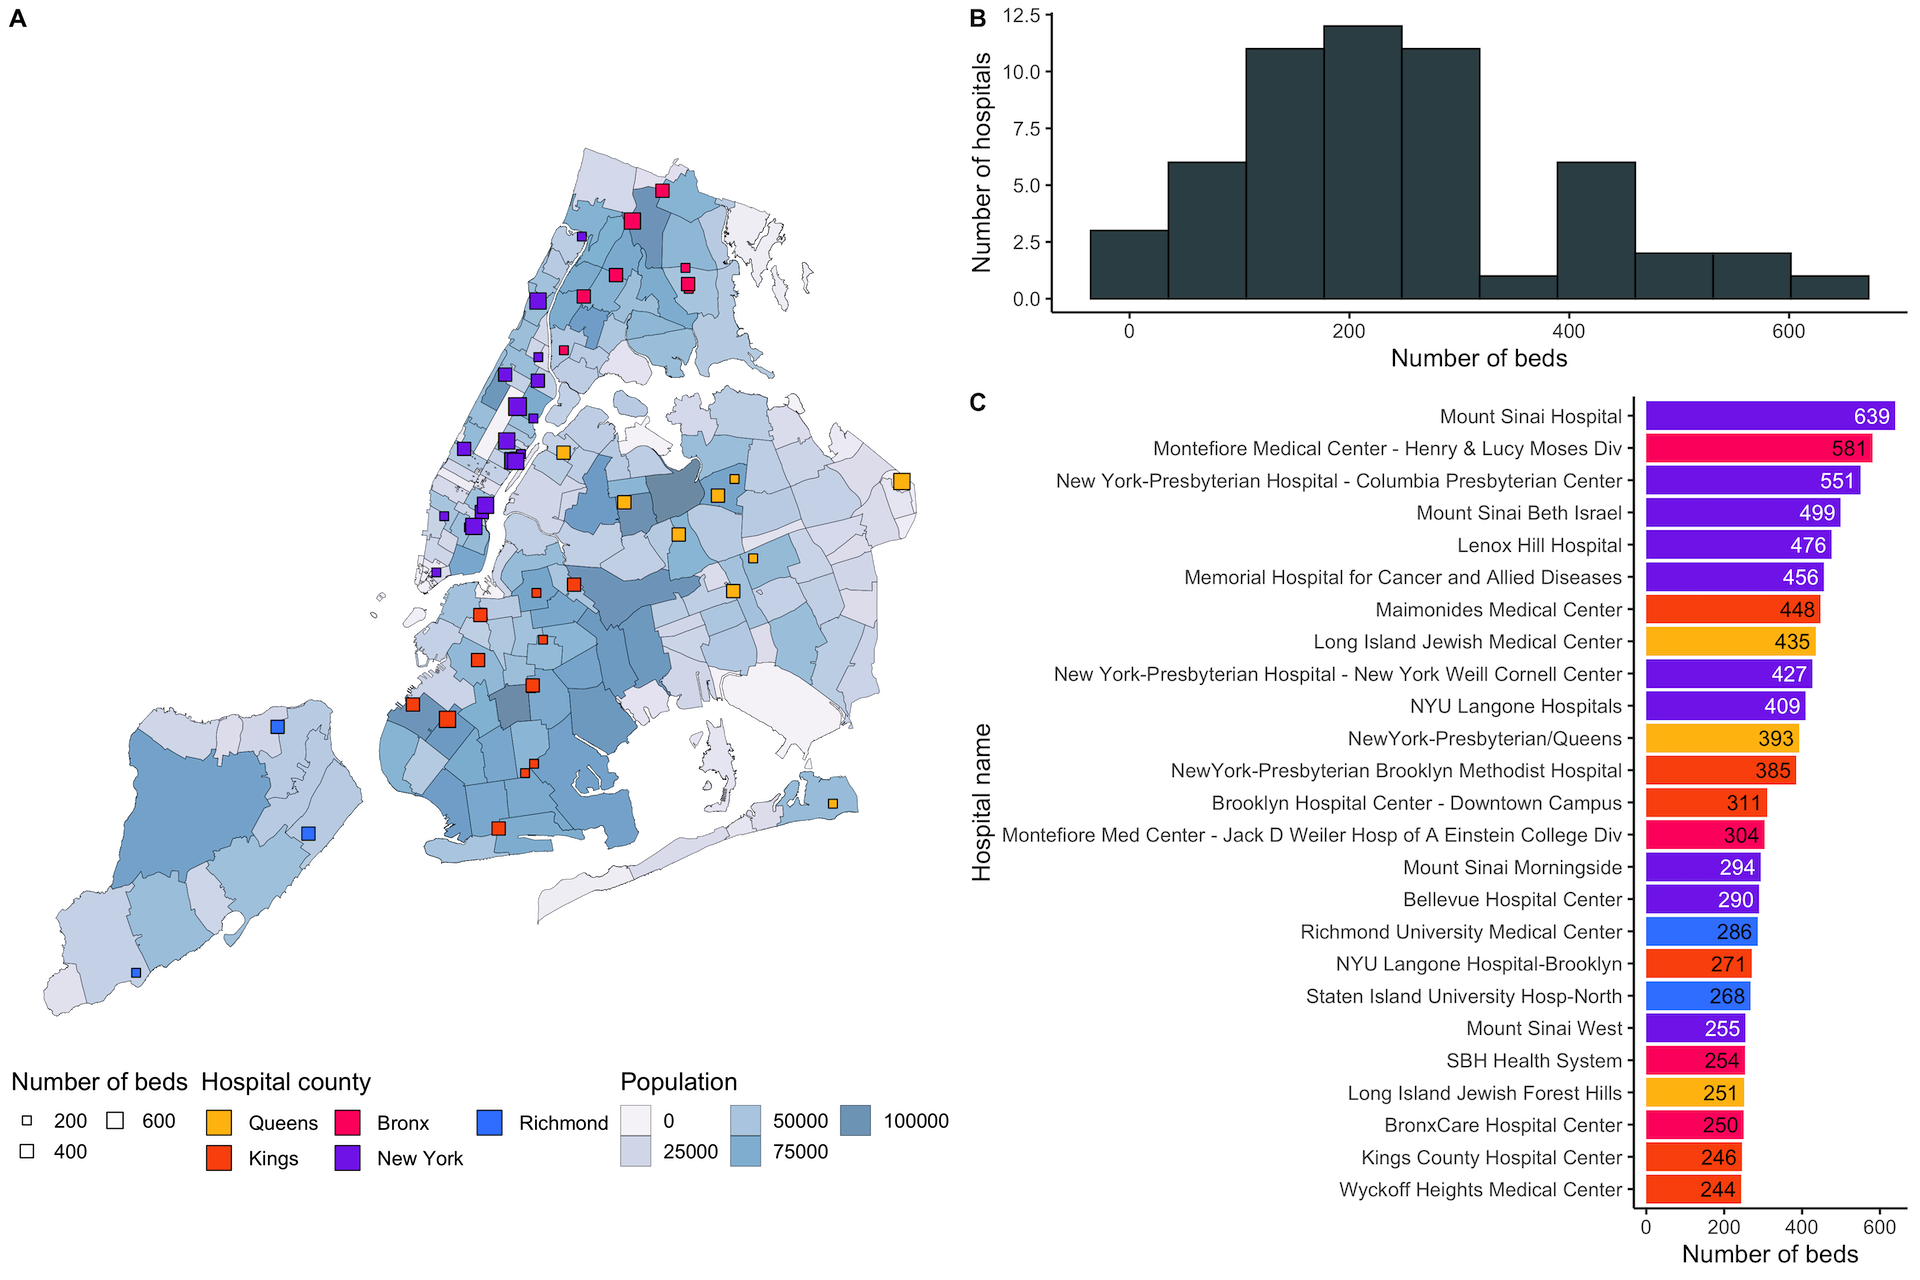
\includegraphics[width=0.9\textwidth]{images/routes/fig1.png}
    \centering
    \caption{ \textbf{Average driving duration for cancer patients in
            metropolitan France.} Map (A) displays the average driving duration by
        municipalities. The median travel duration is higher for municipalities
        with lower population densities (B). The median travel duration is
        especially high for patients from rural areas visiting specialized
        hospitals (C). Patients living in dense areas do not need to travel far
        when reaching specialized hospitals (C). }
    \label{fig:routes-duration-france}
\end{figure}

\subsection{Travel burden index}

For each patient route, we obtained a travel burden score, expressed as a linear
combination between travel duration, travel distance, number of roundabouts and
road sinuosity. The weights are the loading scores of the input variables along
the first principal component of the PCA analysis. The higher the weight is, the
more contribution the input variable has in the component. The loading scores
were: 0.57 for duration; 0.55 for distance; 0.32 for number of roundabouts; and
0.52 for road sinuosity. The median travel burden score was 0.069, ranging
between 0 and 0.98. We discretized the distribution into 5 quantiles with the
following cuts: 0, 0.04; 0.06 0.08; 0.1; 1. The lower the score, the lower the
travel burden is. We discretized the average score into 5 quantiles. For
municipalities in the first quantile, the average travel burden score is in the
top 20\%, meaning that patients travel are shorts and road sinuosity is low.
We studied the travel burden score distribution, and compared it to the input
variables (\cref{fig:routes-burden-distribution}). The score has a strong
positive correlation with road sinuosity (0.89); duration (0.85);
distance (0.8); and number of roundabouts (0.68). The municipalities
median revenue and population densities were lightly negatively correlated,
with coefficients of -0.29 and -0.09 respectively (C). We compared the travel
duration, distance, sinuosity and score on plots (D) and (E). As expected,
we notice that travels in the lowest quantiles have low duration and distance.
However, at a given travel distance, increasing the travel duration will result
in a score increase (D). Travel duration exponentially increase with the road
sinuosity (E), and high sinuosity values correspond to higher travel burden
quantiles.

\begin{figure}[h!]
    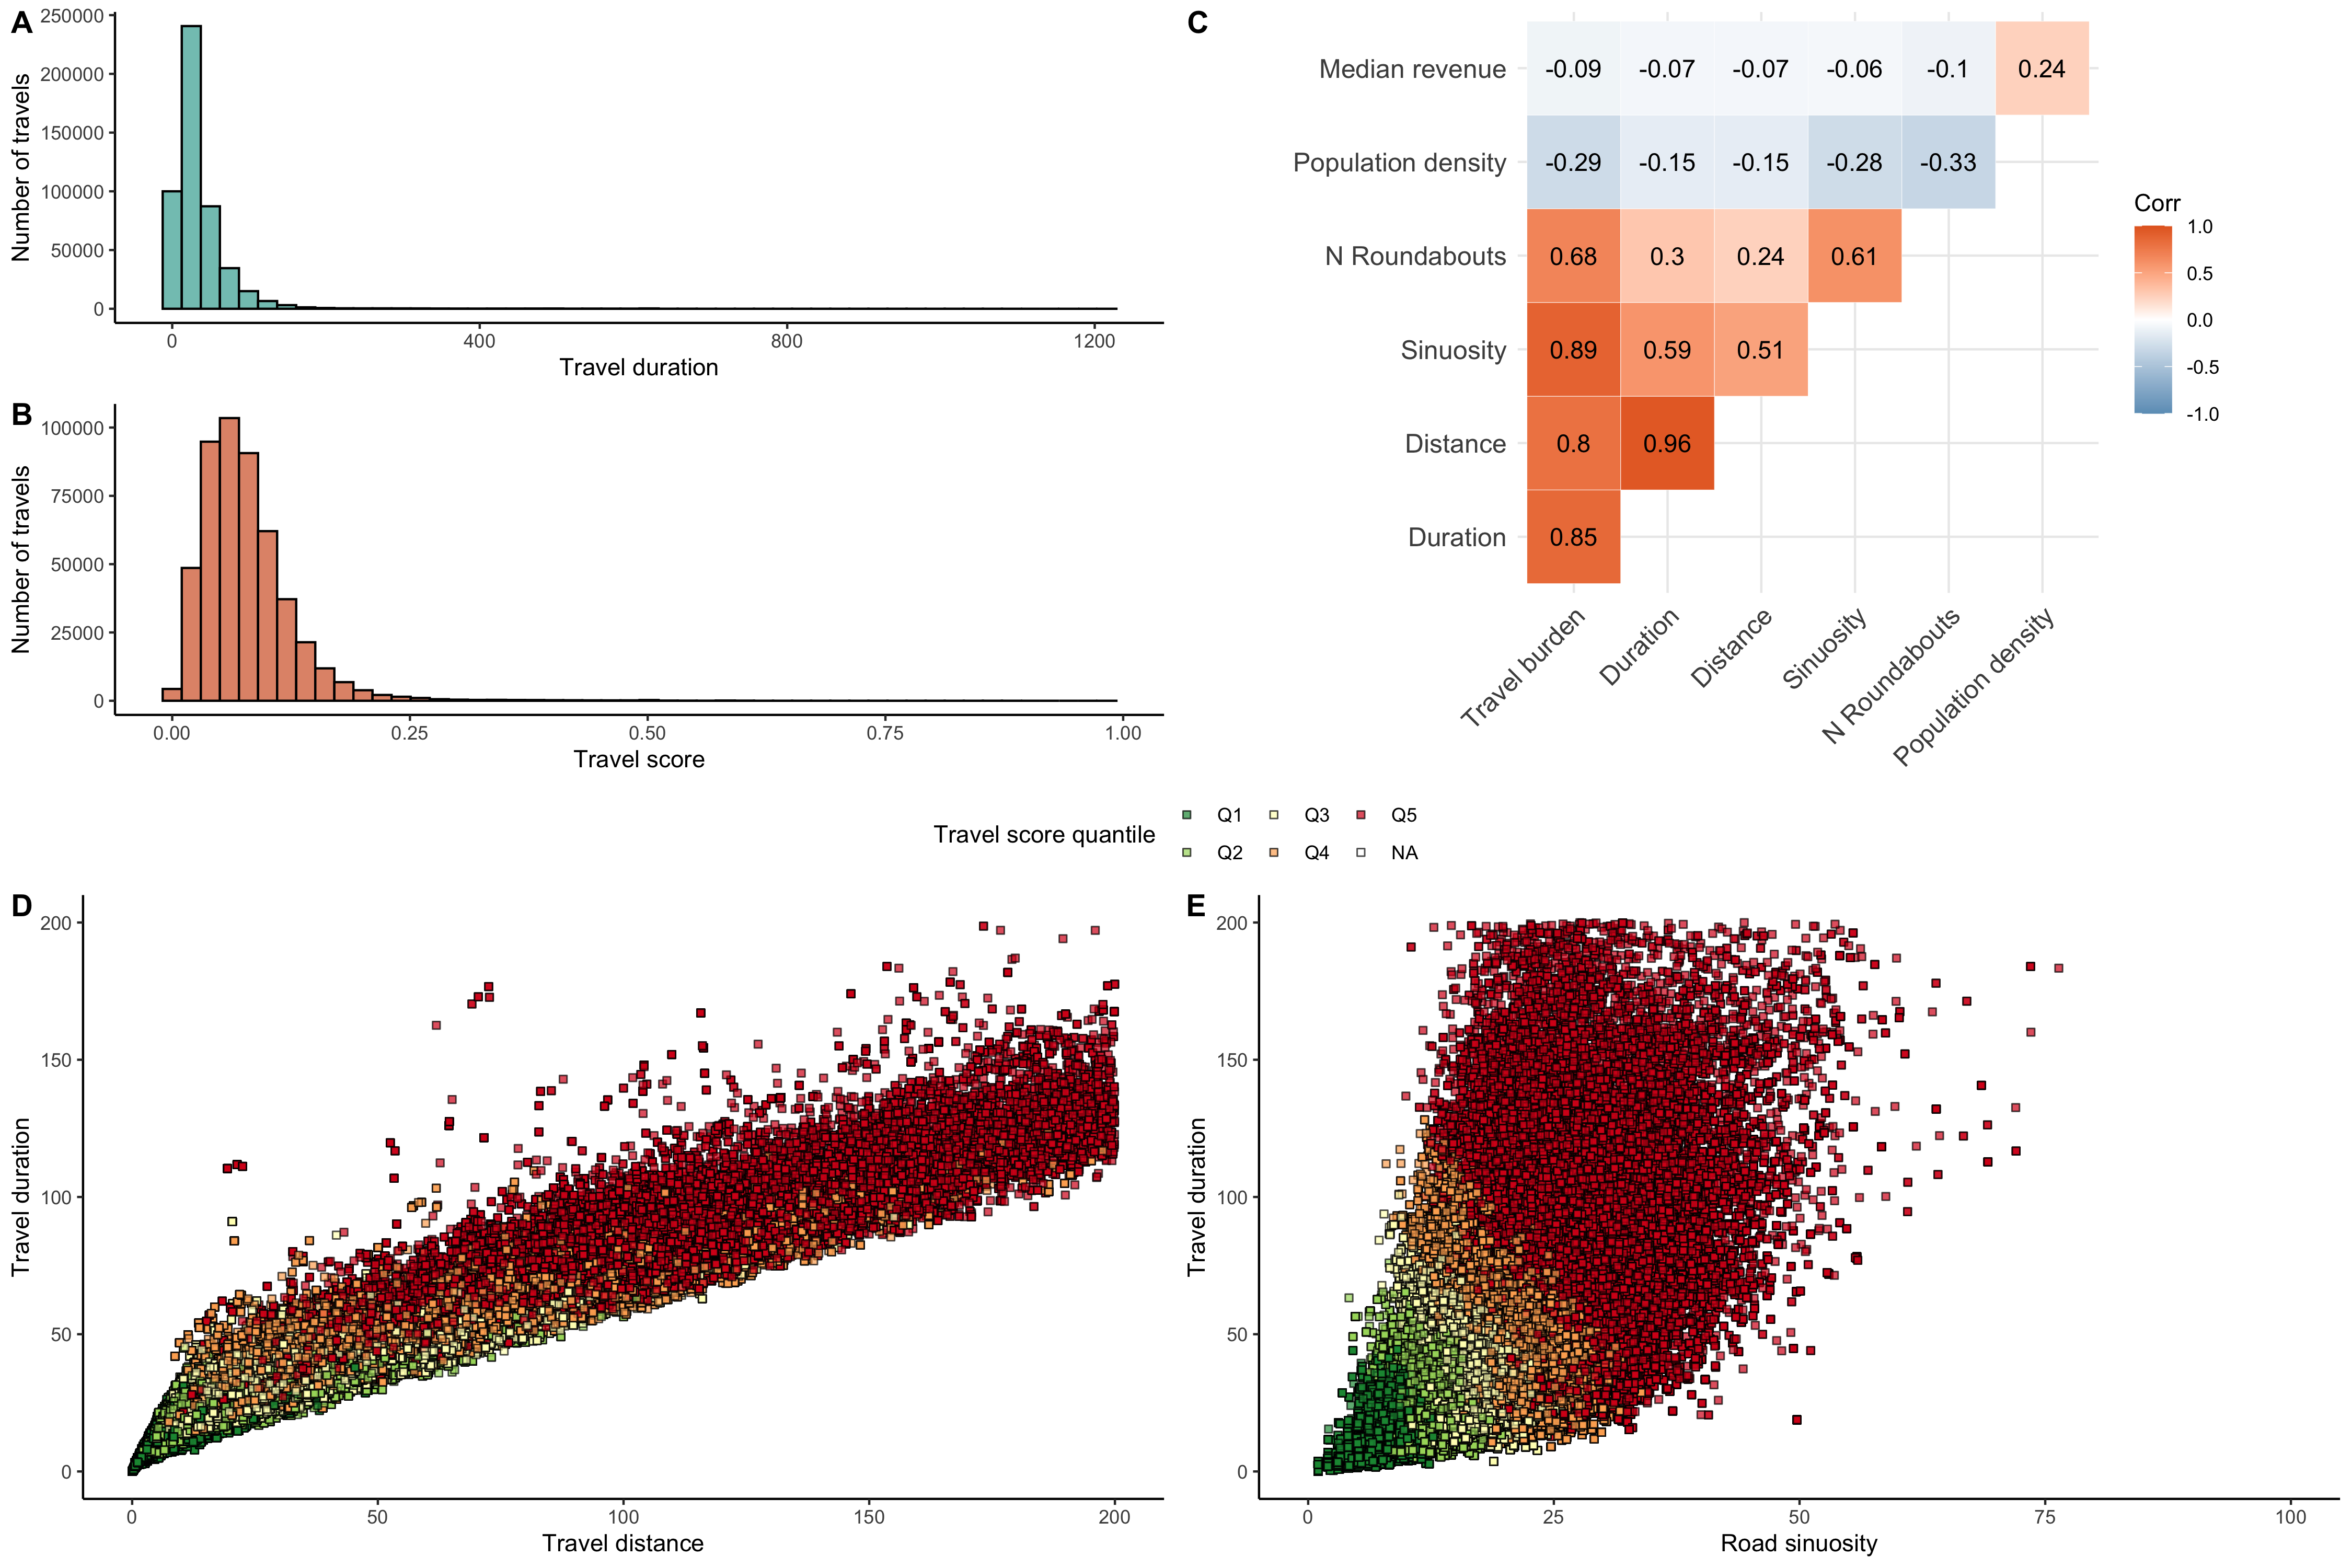
\includegraphics[width=0.9\textwidth]{images/routes/sup_fig_3.png}
    \centering
    \caption{
        \textbf{Travel burden score distribution per department and region.}
        Comparison between travel duration distribution (A) and travel burden
        distribution (B). Correlations between travel burden score and other
        variables (C). Comparison between travel distance, duration, and travel
        score (D). Comparison between road sinuosity, travel duration and travel
        score (E).}
    \label{fig:routes-burden-distribution}
\end{figure}

We now study the spatial distribution of the travel burden score, by displaying
the average travel burden score per municipality on a map
(\cref{fig:routes-burden-index}-A). The municipalities are filled by median
driving duration, discretized according to the previously stated quantiles.
We notice spatial disparities in the distribution. Areas with high travel
burden are mostly located in regions like Corse, Pays de la Loire, Occitanie
and Provence-Alpes-Cote-d'Azur. In general, municipalities with lower
population densities have a higher number of routes with high travel burden (C).
For instance, among all the municipalities with population densities lower than
30 inhabitants per km\textsuperscript{2} 40.2\% are in the worst quantile,
compared to only 11.3\% for municipalities with 200 or more inhabitants per
km\textsuperscript{2} (B).

\begin{figure}[h!]
    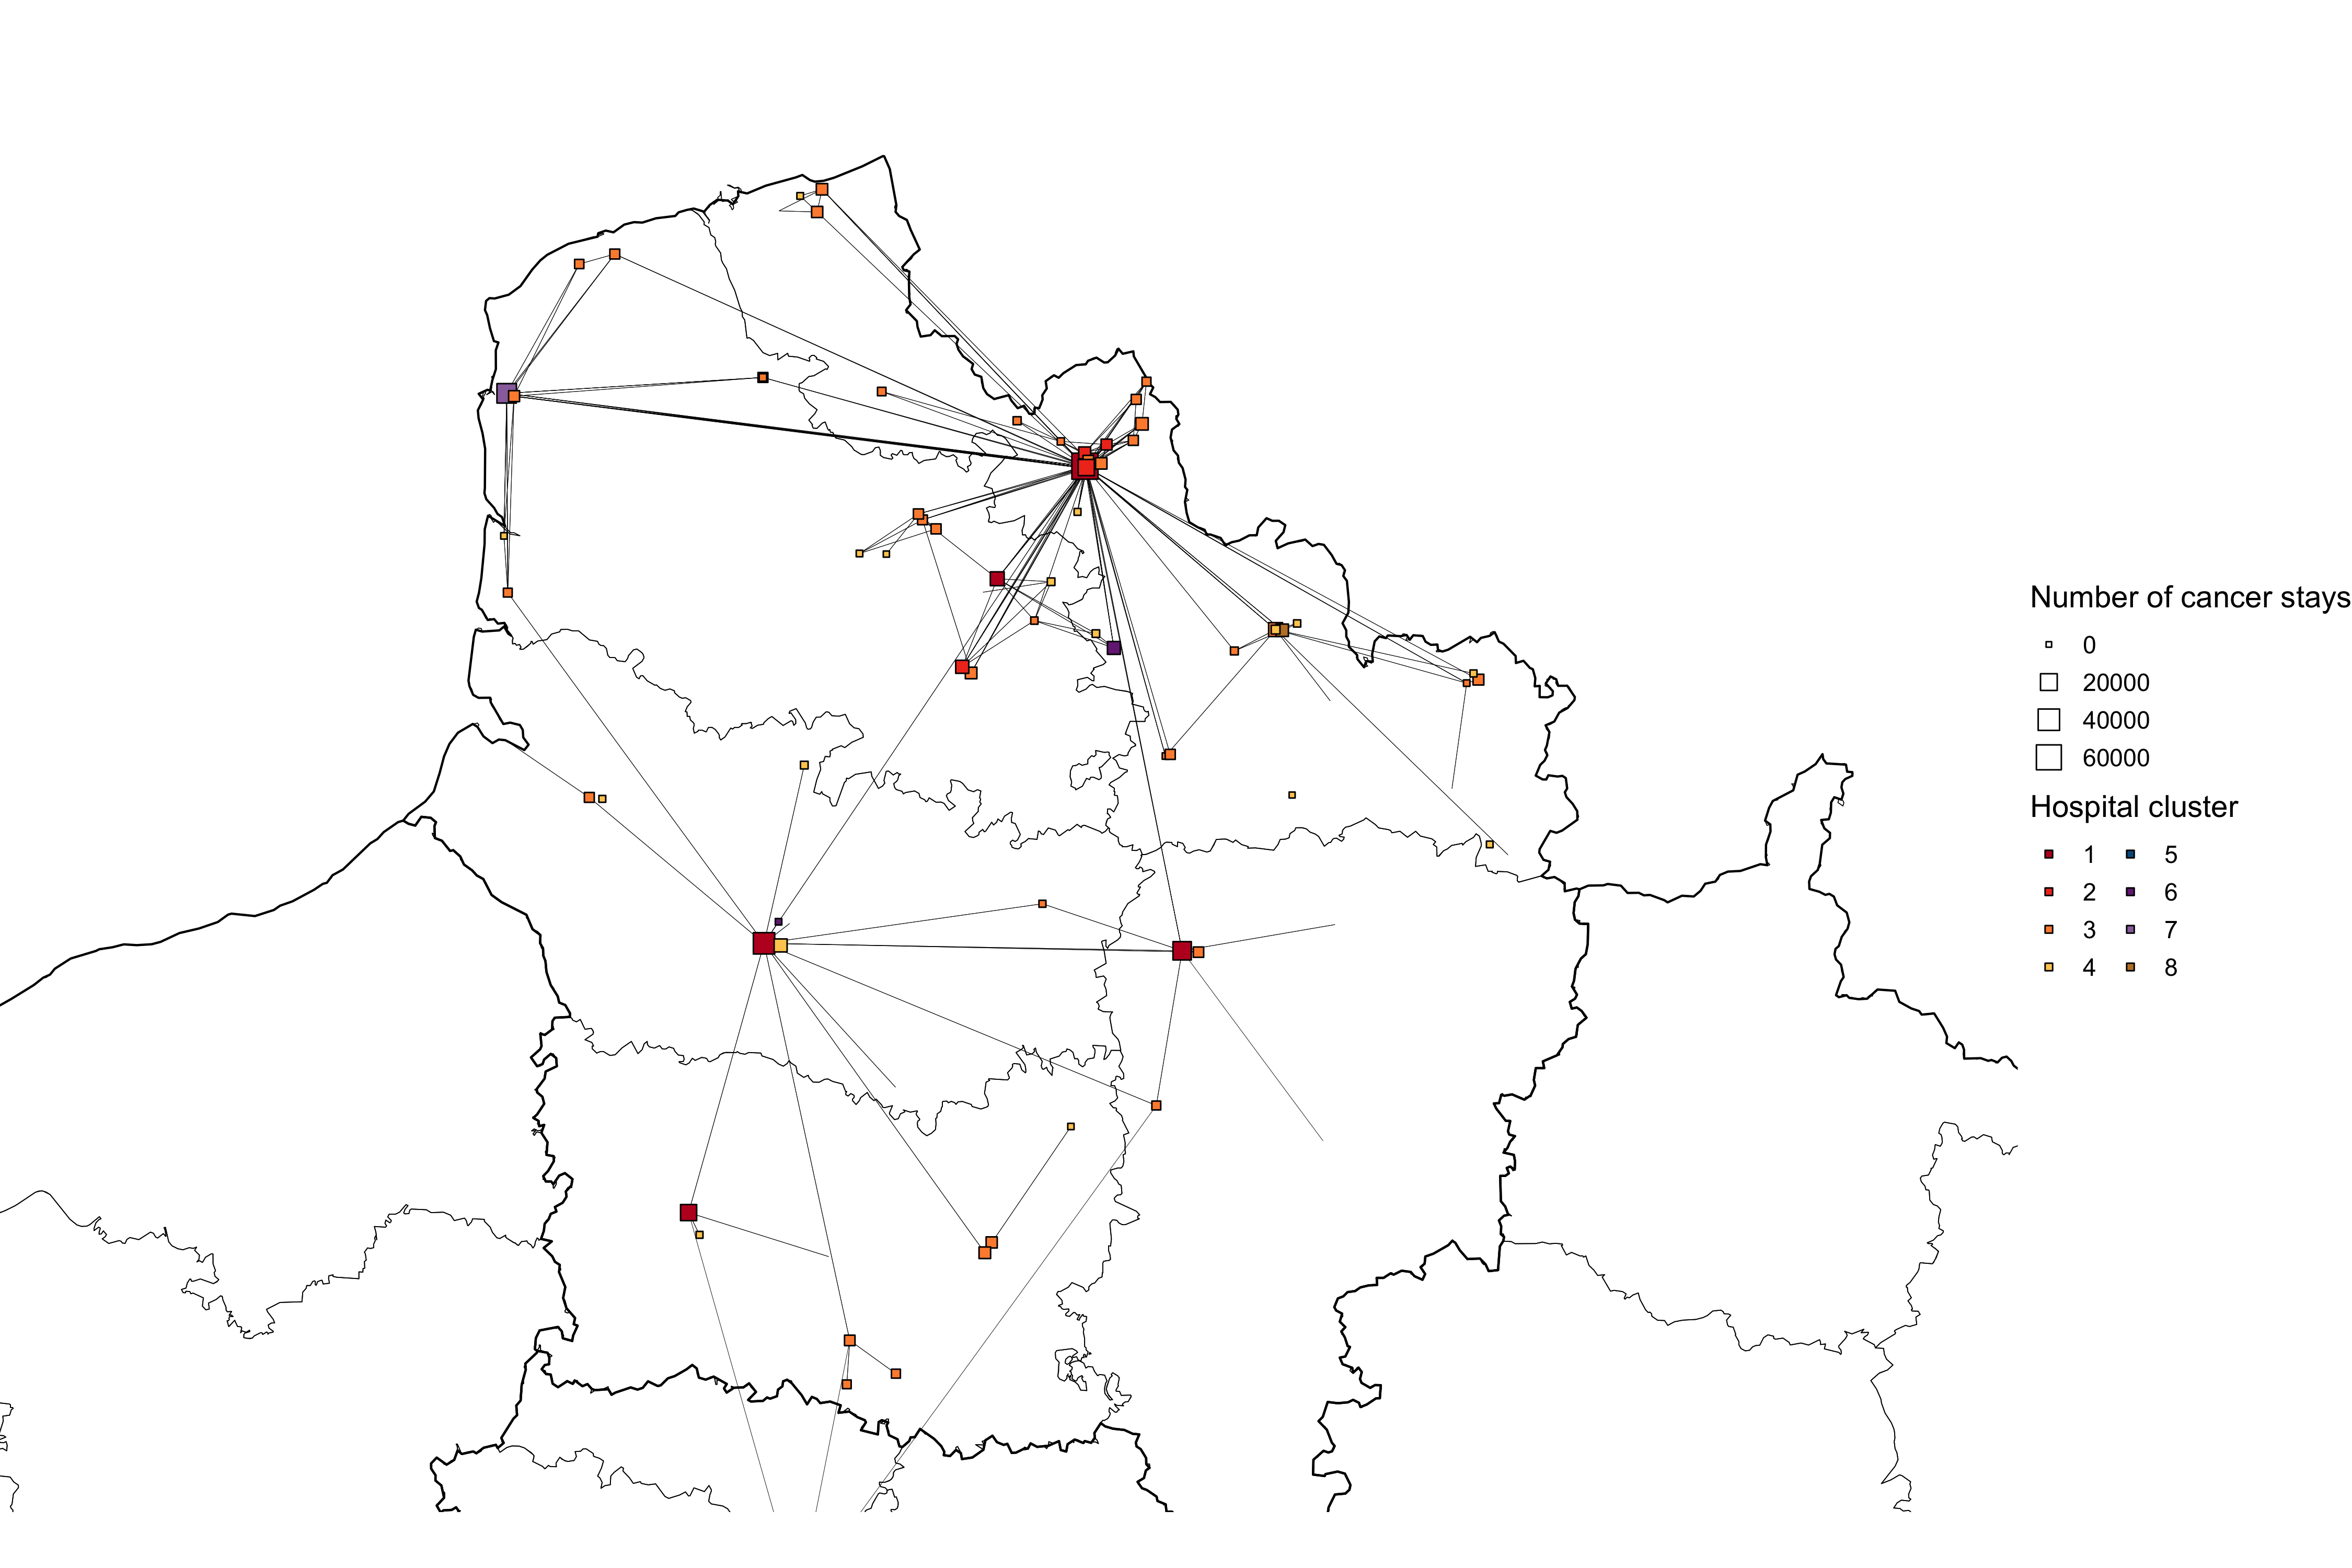
\includegraphics[width=0.9\textwidth]{images/routes/fig2.png}
    \centering
    \caption{
        \textbf{Travel burden index in metropolitan France.}
        The travel burden index is a composite score based on route duration,
        distance, number of roundabouts and sinuosity. The higher the score is,
        the more tedious the route is. The score distribution is displayed on
        map (A). The percentage of routes with higher scores increases in lower
        density areas (B). Figure (C) displays the input variables median values
        by score quantiles. For instance, the median road sinuosity is much
        higher when the score is high. }
    \label{fig:routes-burden-index}
\end{figure}

The travel burden index varied from a region to another, especially in the most
rural departments. We ranked the regions by median travel burden index in
increasing order and obtained the following: Île-de-France (median=0.0477,
sd=0.0377); Normandie (median=0.0649, sd=0.0440); Hauts-de-France
(median=0.0681, sd=0.0405); Bretagne (median=0.0691, sd=0.0428);
Provence-Alpes-Côte d'Azur (median=0.0701, sd=0.0476); Grand Est (median=0.0709,
sd=0.0409); Auvergne-Rhône-Alpes (median=0.0725, sd=0.0492);
Bourgogne-Franche-Comté (median=0.0757, sd=0.0466); Nouvelle-Aquitaine
(median=0.0773, sd=0.0520); Centre-Val de Loire (median=0.0795, sd=0.0440); Pays
de la Loire (median=0.0812, sd=0.0469); Occitanie (median=0.0816, sd=0.0523);
Corse (median=0.147 , sd=0.188). The 5 departments which had the lower median
travel burden index were Paris, Val-de-Marne, Hauts-de-Seine, Seine-St-Denis,
and Rhone. Among these departments, the first 4 are in Ile de France region. The
5 departments with the highest travel burden are from lowest to highest:
Aveyron, Corse-du-Sud, Lozère, Ardèche, and Haute-Corse
(\cref{fig:routes-burden-departments-top-bottom-20}).

\begin{figure}[h!]
    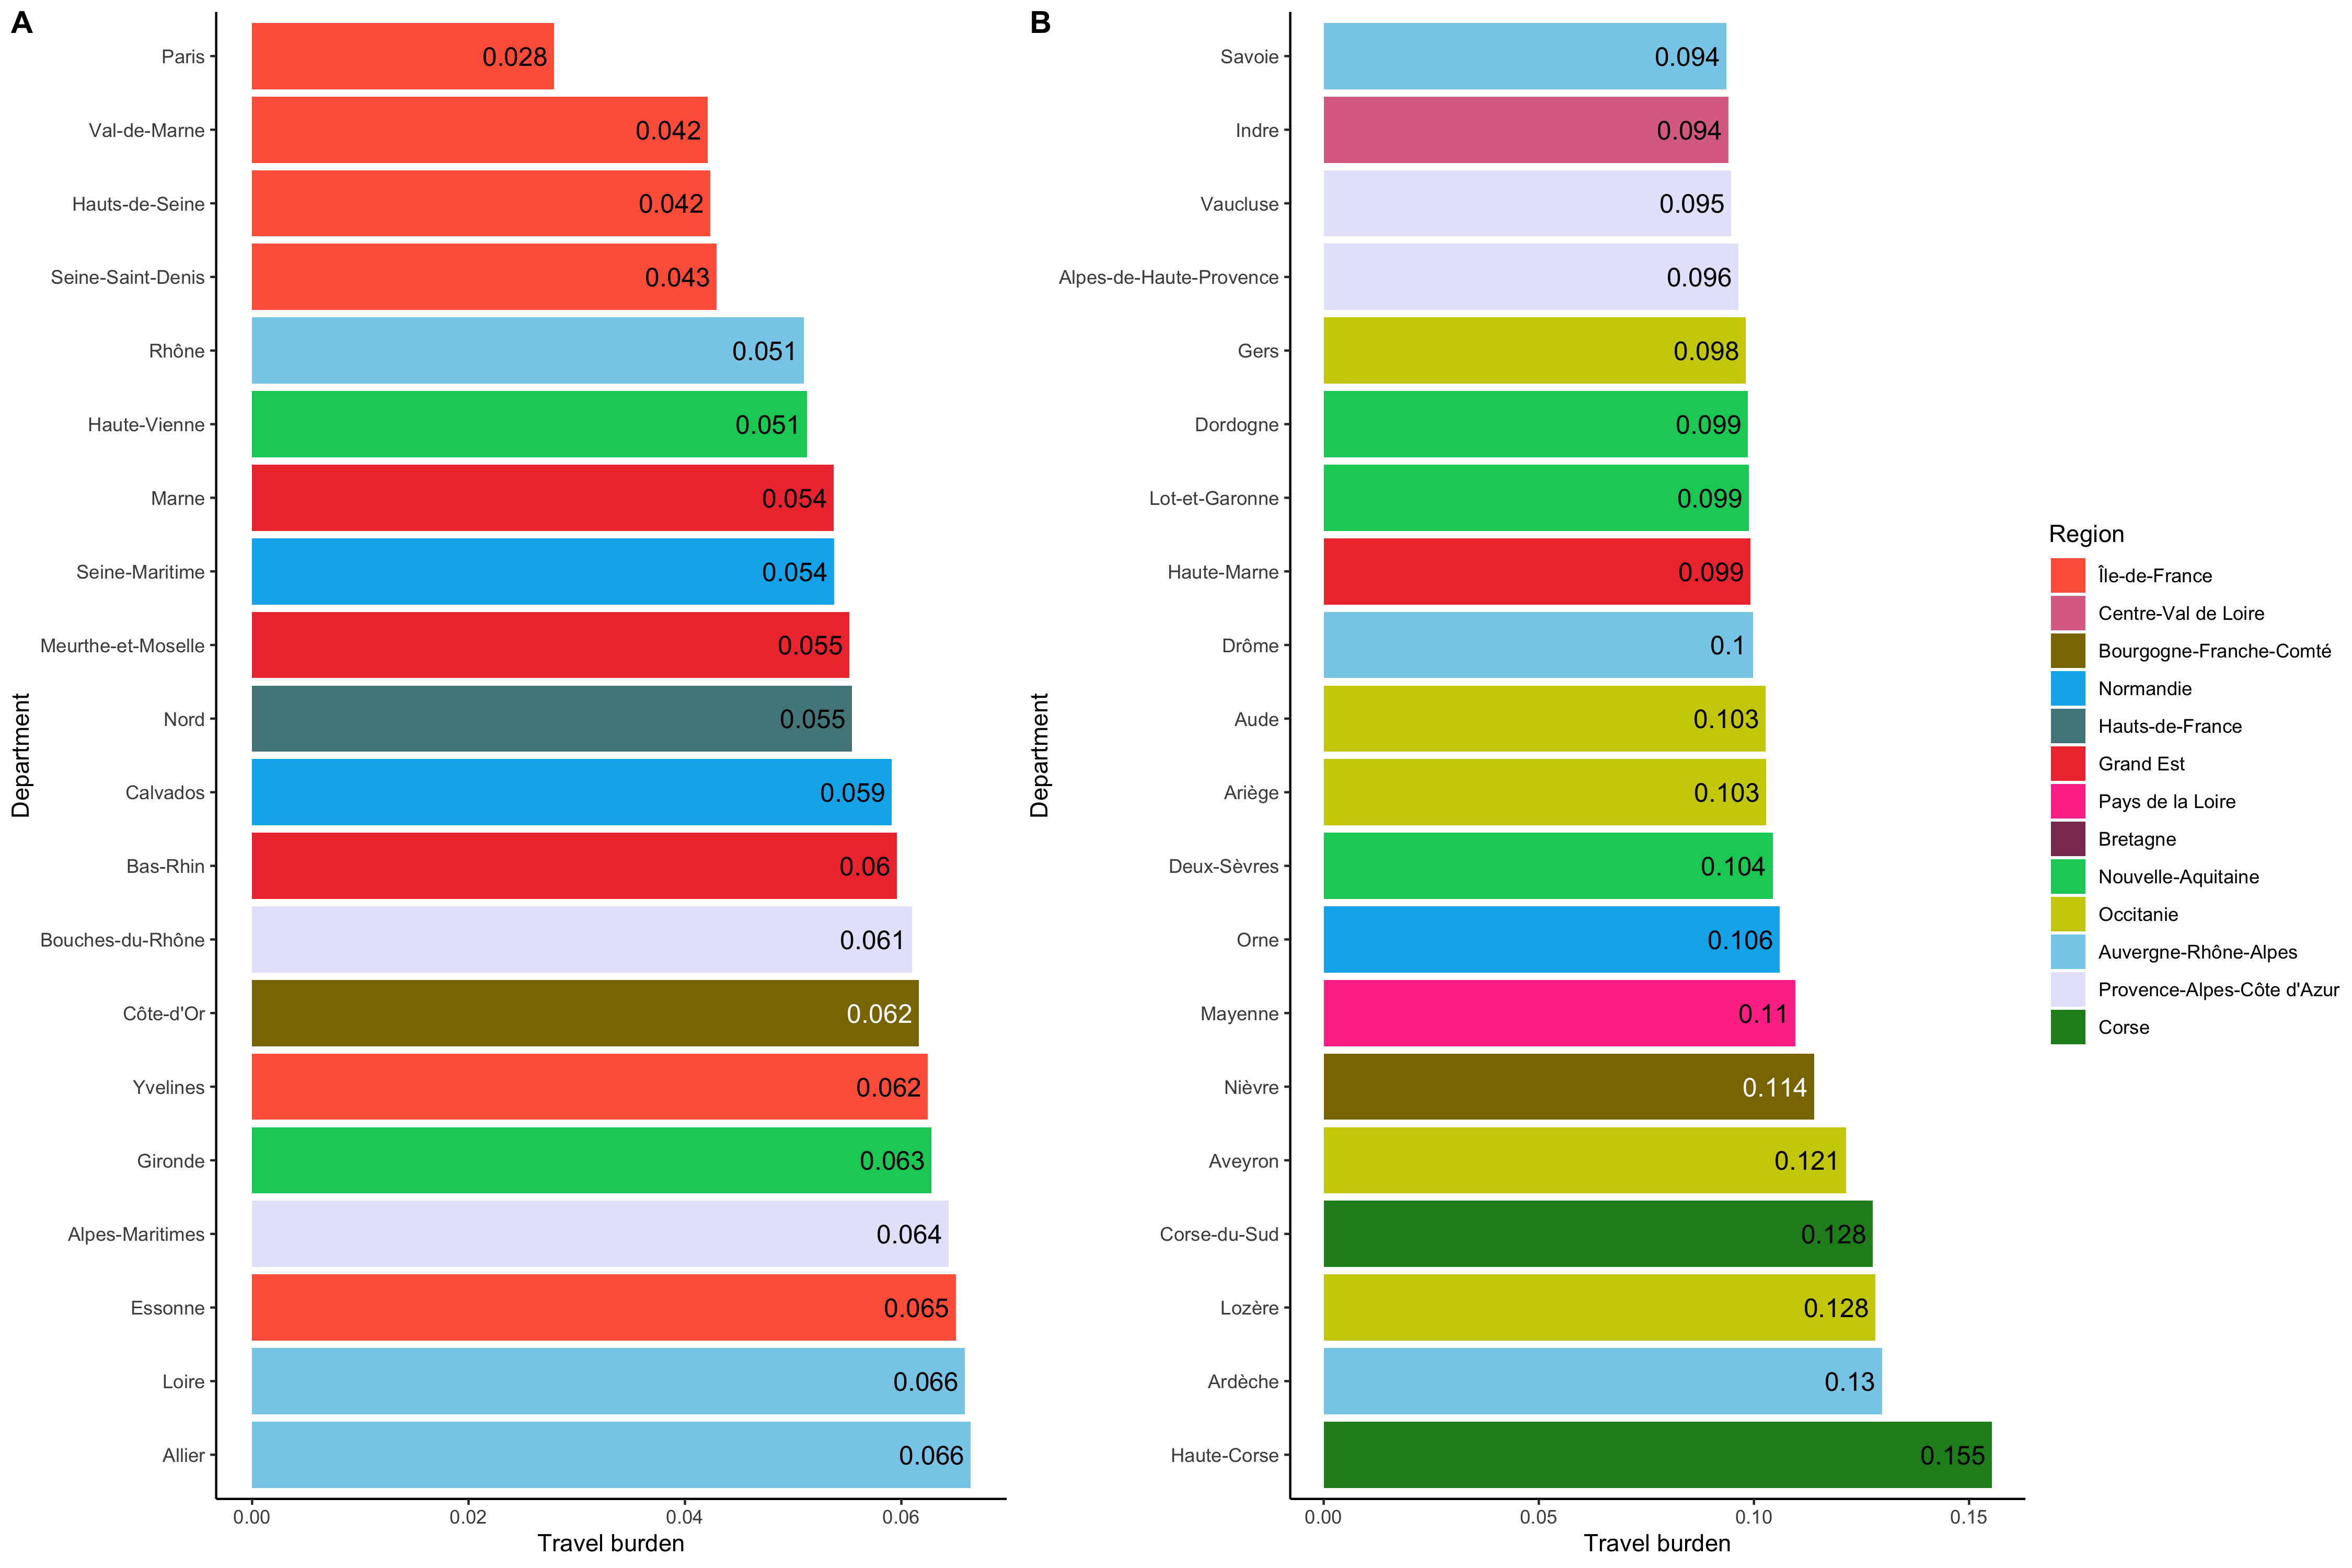
\includegraphics[width=0.9\textwidth]{images/routes/sup_fig_2.png}
    \centering
    \caption{
        \textbf{Travel burden score distribution per department and region.}
        The 5 departments which had the lower median travel burden index were
        Paris, Val-de-Marne, Hauts-de-Seine, Seine-St-Denis, and Rhone. Among these
        departments, the first 4 are in Ile de France region. The 5 departments with the
        highest travel burden are from lowest to highest: Aveyron, Corse-du-Sud, Lozère,
        Ardèche, and Haute-Corse}
    \label{fig:routes-burden-departments-top-bottom-20}
\end{figure}

We then focused on a single region, and compared the average travel burden score
with the main roads location, as illustrated on \cref{fig:travel-burden-paca}.
We did not show the roads that with were used by less than 5 patients during the
year, for clarity. In this region, we recall that the two largest cities are
Marseille and Nice, and that the accessibility is the highest along the
coastline, where the higher population densities are. The road network is the
most developed on the coastline, as well as around cities like Avignon and Gap.
The areas that had low accessibility scores have high travel burden scores,
which makes sense since the travel burden score was party computed with the
travel duration to reach the hospitals. However, we notice that some areas that
had decent accessibility scores can have average or high average travel burden
scores. This is probably due to the sinuosity of the roads, notably in the Var
department, or in the north of Nice city. The roads in these areas are often
small, with a lot of turns and roundabouts, increasing the travel tediousness.
Overall, the travel burden score is lower for municipalities near the main
roads.

\begin{figure}[h!]
    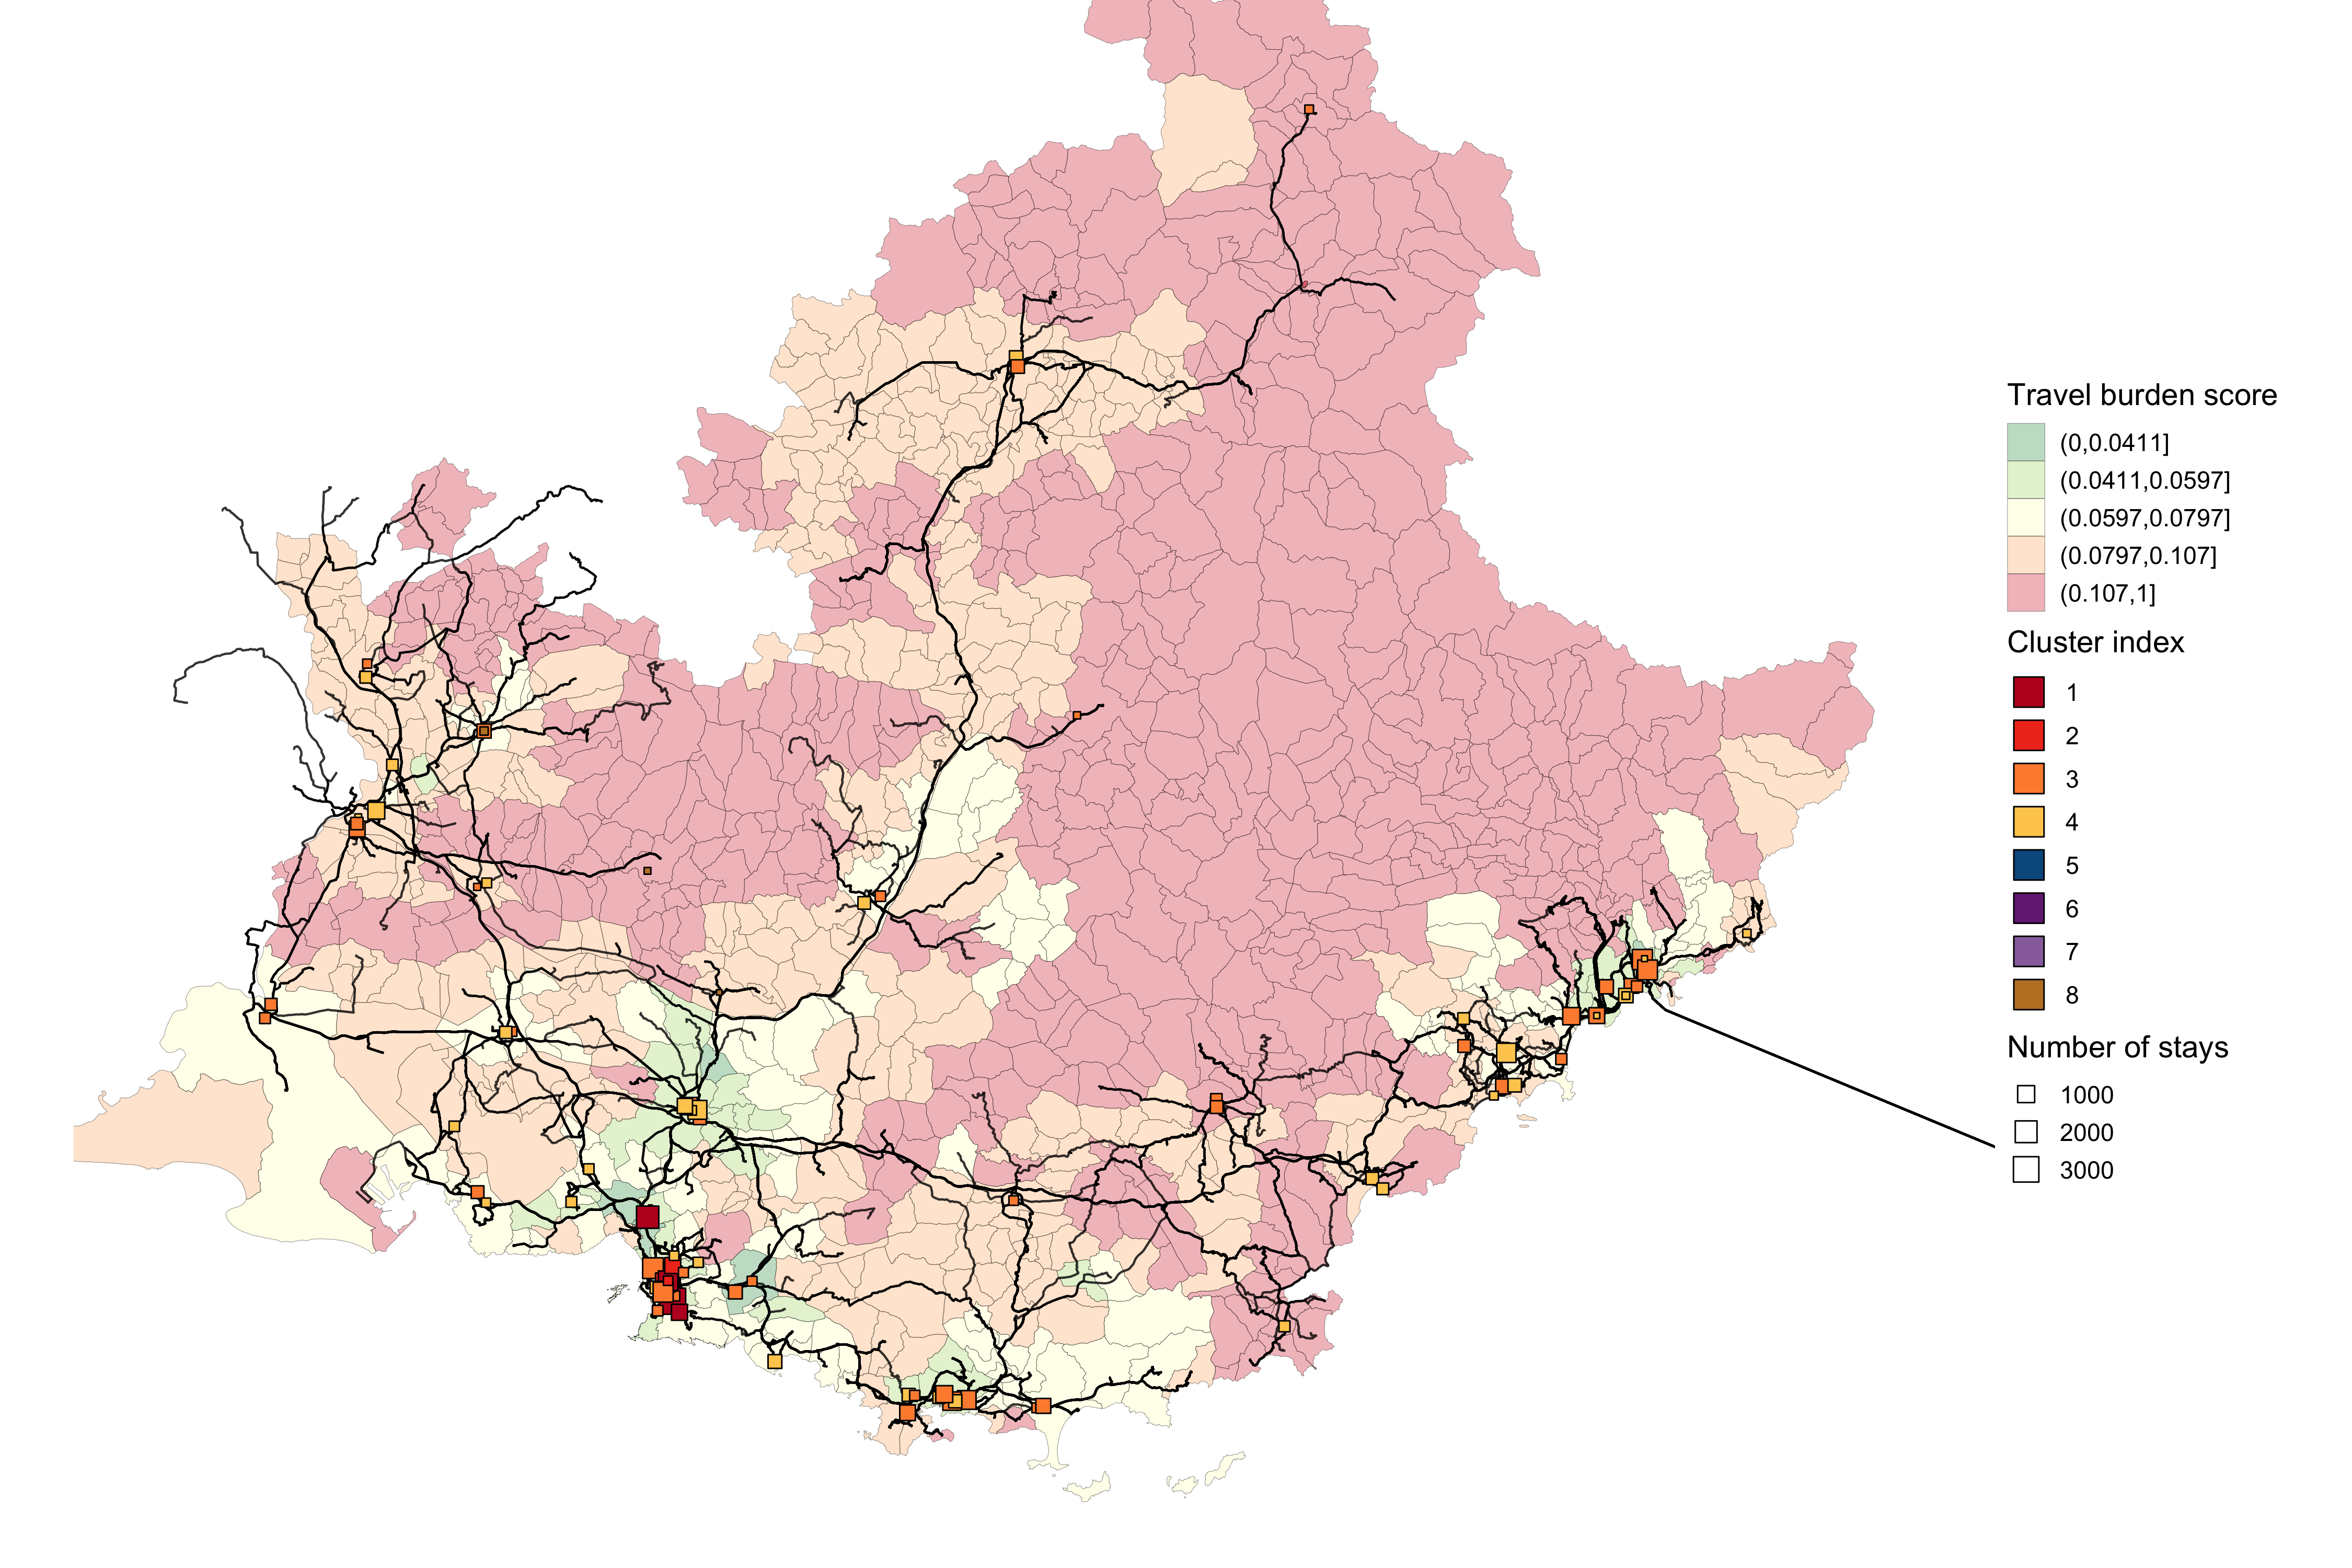
\includegraphics[width=0.9\textwidth]{images/routes/fig7.png}
    \centering
    \caption{
        \textbf{Travel burden score in Provence Alpes Cote d'Azur (PACA) region.}
        We compared the average travel burden score with the main roads
        location. The roads that with were used by less than 5 patients during
        the year are hidden. The areas that had low accessibility scores have
        high travel burden scores. However, we notice that some areas that had decent
        accessibility scores can have average or high average travel burden
        scores. This is probably due to the sinuosity of the roads, notably in
        the Var department, or in the north of Nice city. The roads in these
        areas are often small, with a lot of turns and roundabouts, increasing
        the travel tediousness. }
    \label{fig:travel-burden-paca}
\end{figure}

\subsection{Carbon footprint of patients travel}

The overall carbon emissions associated with the included travels in this study
was 2,159 tons of \ac{co2}. The total emissions per cancer type vary between 373
tons for malignant tumors of the digestive organs, and 20 tons for malignant
tumors of bone and articular cartilage. Despite being the cancer type with the
most stays, malignant melanoma and skin tumors do not represent the highest
carbon footprint (\cref{fig:carbon-footprint-pathology}). Indeed, the 104,429
stays in this pathology are associated with 360 tons of \ac{co2} emissions;
where the 81,440 stays related to malignant tumors of digestive organs are
associated with 373 tons of emitted \ac{co2}. The three cancer types with the
most stays represent nearly 50\% of the overall carbon emissions.

\begin{figure}[h!]
    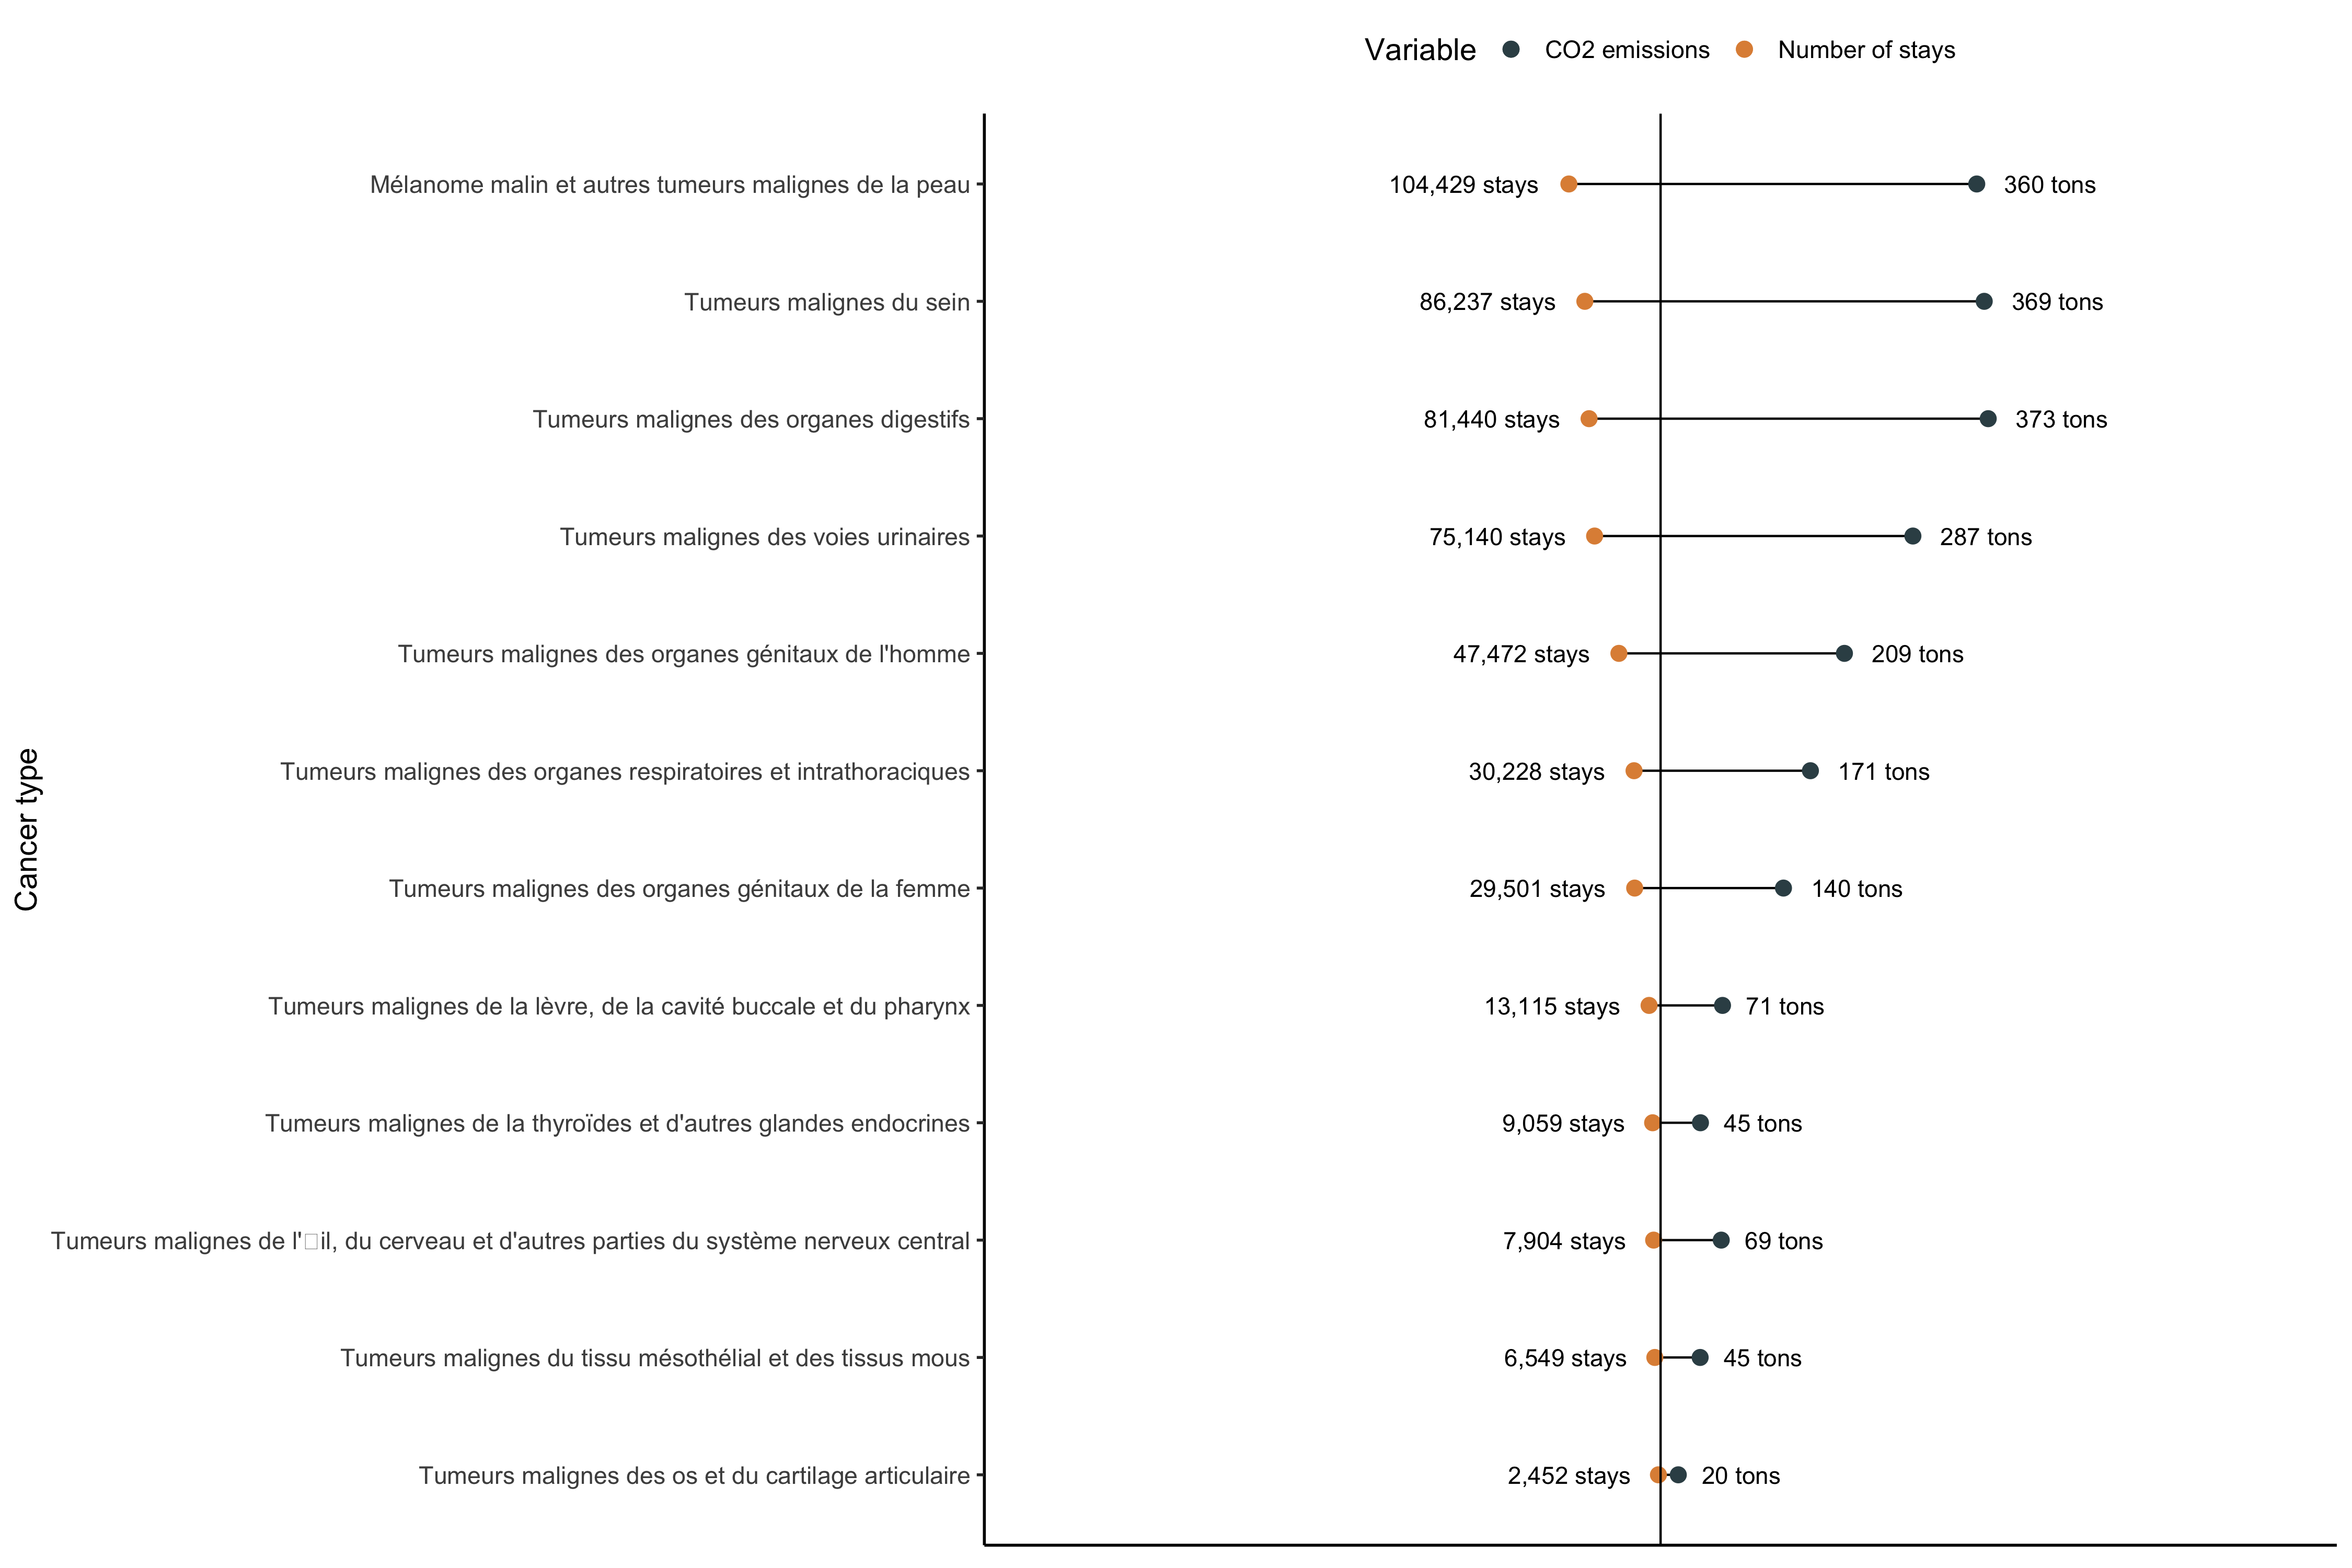
\includegraphics[width=0.9\textwidth]{images/routes/fig12.png}
    \centering
    \caption{
        \textbf{Carbon footprint and number of stays by cancer location}
        The total emissions per cancer type vary between 373 tons for
        malignant tumors of the digestive organs, and 20 tons for malignant tumors
        of bone and articular cartilage.}
    \label{fig:carbon-footprint-pathology}
\end{figure}

The average \ac{co2} emissions per travel increased with the rarity of the
cancer and the scarcity of hospitals habilitated to treat this disease
(\cref{fig:avg-carbon-footprint-pathology}). Indeed, the average \ac{co2}
emissions were the lowest for malignant melanoma and other malignant skin
tumors, which had the highest amount of stays (A) and specialized hospitals
(B). The rare cancers like bone or eye cancer had the highest average
carbon emissions.

\begin{figure}[h!]
    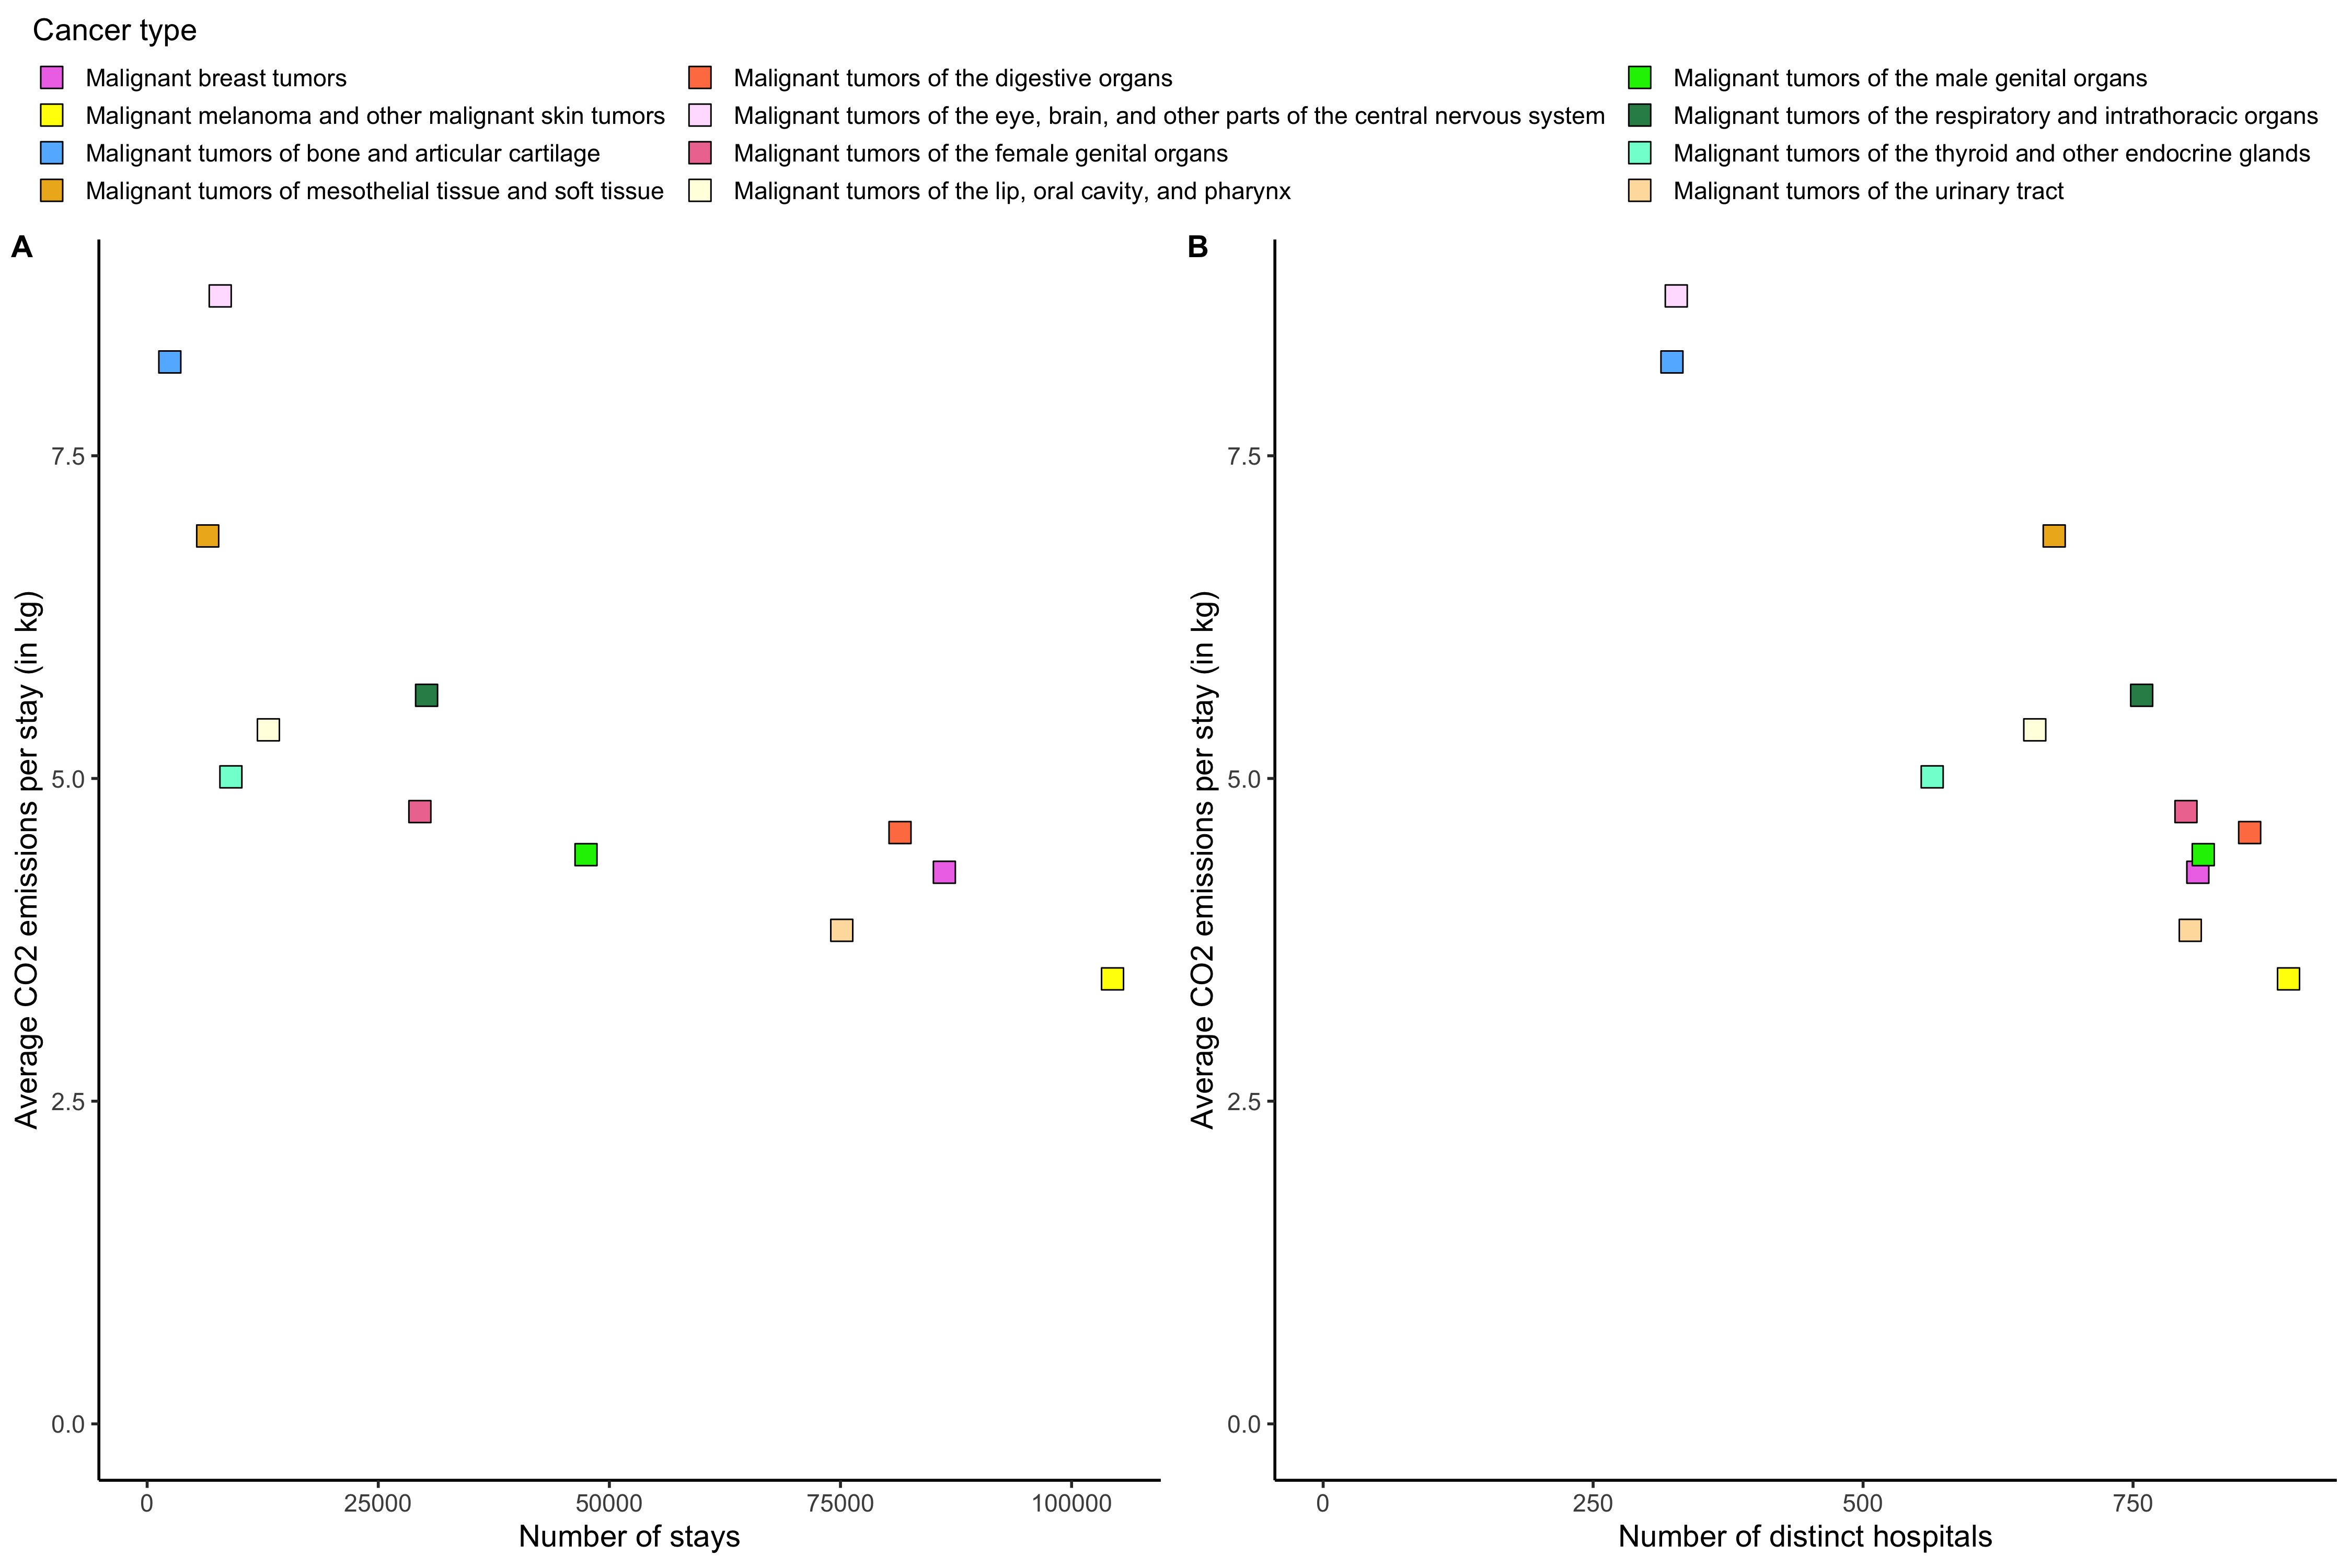
\includegraphics[width=0.9\textwidth]{images/routes/sup_fig_4.png}
    \centering
    \caption{ \textbf{Average carbon footprint by cancer location.} Comparison
        between the average \ac{co2} emissions and the number of stays (A), as
        well as with the number of habilitated hospitals (B). The average
        \ac{co2} emissions per travel increased with the rarity of the cancer
        and the scarcity of hospitals habilitated to treat this disease. }
    \label{fig:avg-carbon-footprint-pathology}
\end{figure}

The average emissions of \ac{co2} vary depending on the oncology specialization
of the visited hospital, and the rurality of the patient municipality of
residence. Regardless of the cancer site, the average emissions for patients
visiting hospitals from the most specialized cluster was 6.05 kg, versus 3.84 kg
and 3.42 kg for hospitals within clusters 3 and 4
(\cref{fig:avg-carbon-footprint-density-cluster}-A). Similarly, the average
emissions for patients living in municipalities with less than 30 inhabitants
per km\textsuperscript{2} was 8.1 kg, compared with 2.9 kg for municipalities
with > 200 inhabitants per km \textsuperscript{2}
(B). Finally, the average emissions were the highest for patients living
in the least densely populated areas, and visiting the most specialized
hospitals (C). The emissions are 11.1 kg on average for patients living in
< 30 inhabitants per km \textsuperscript{2} and visiting hospitals within
cluster 1.

\begin{figure}[h!]
    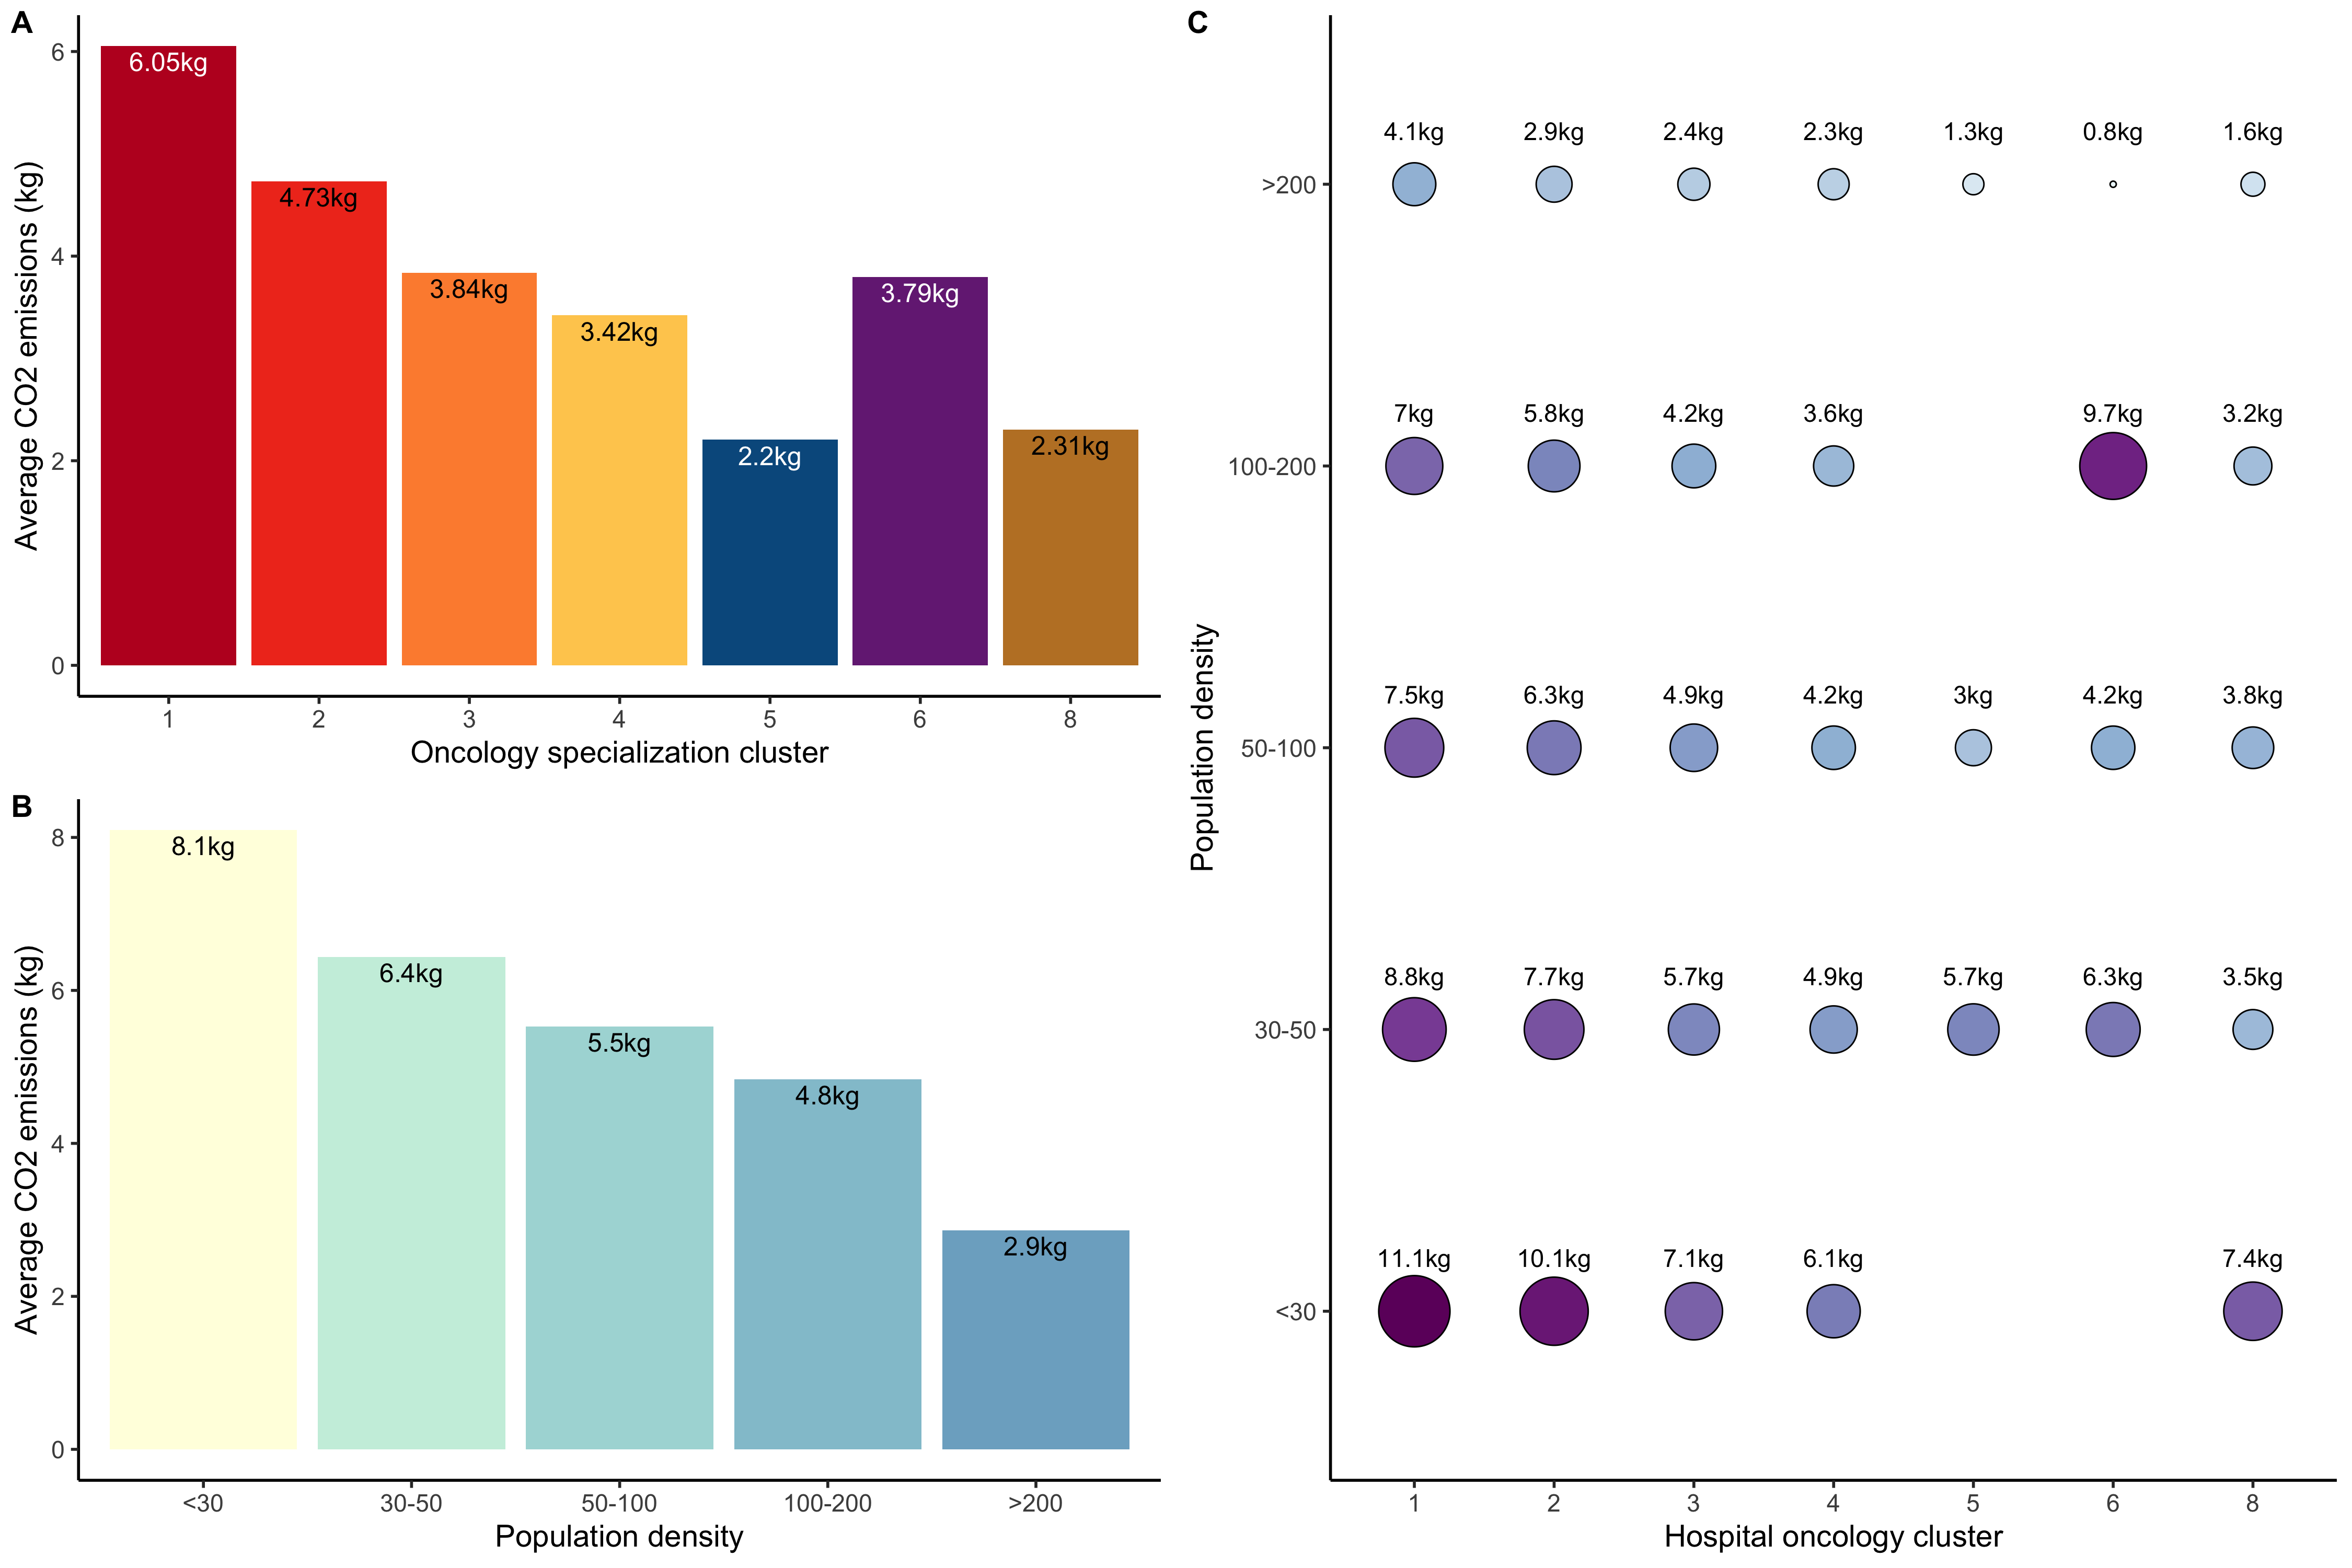
\includegraphics[width=0.9\textwidth]{images/routes/sup_fig_5.png}
    \centering
    \caption{ \textbf{Average carbon footprint according to the hospital
            oncology specialization and municipality population density.} Regardless
        of the cancer site, the average \ac{co2} emissions are higher for
        patients visiting the most specialized hospitals (A). Similarly,
        the emissions are higher for patients living in rural areas (B).
        Finally, the average emissions are the highest for patients living in
        rural municipalities and visiting the most specialized hospitals (C).}
    \label{fig:avg-carbon-footprint-density-cluster}
\end{figure}

We now focus on a single department and chose Ain, in Auvergne-Rhone-Alpes
region. The largest city in Ain is Bourg-en-Bresse, with a population of 41,248
inhabitants in 2018; and a population density of 1,729 inhabitants per km
\textsuperscript{2}. The Ain department is mostly populated with sub-urban and
rural municipalities, but it is located near the Rhone department, where urban
municipalities are, including Lyon, the third largest city in the country. We
analyzed the travels frm patients living in municipalities from the Ain
department, and shown which hospitals they visited on
\cref{fig:routes-co2-emissions}. The alluvium chart on sub-figure (A) displays
the number of patients routes between municipalities on the left and hospitals
on the right. The alluvium flows are sized by number of stays and colored by the
stays carbon footprint. The darker flows indicate higher \ac{co2} emissions. We
point that the routes with the more emissions are not necessarily the routes
with the most patients. To illustrate this, we show the total \ac{co2} emissions
per visited hospital for patients living in Bourg-en-Bresse (B).
Centre-Hospitalier de Fleyriat is the most visited hospitals among patients
living in Bourg-en-Bresse, with 150 stays and 4-kilometer distance between the
municipality centroid and the hospital. The resulting \ac{co2} emissions are 72
kg. However, some patients are traveling outside of Bourg-en-Bresse to reach
hospitals based in Lyon, which represents at least an 80 km drive. For instance,
there were 18 stays in Hospital Lyon Sud, located at 91 km from Bourg-en-Bresse.
The resulting \ac{co2} emissions were 184 kg, which is more than twice the
emissions of the 150 stays in CH Fleyriat.

\begin{figure}[h!]
    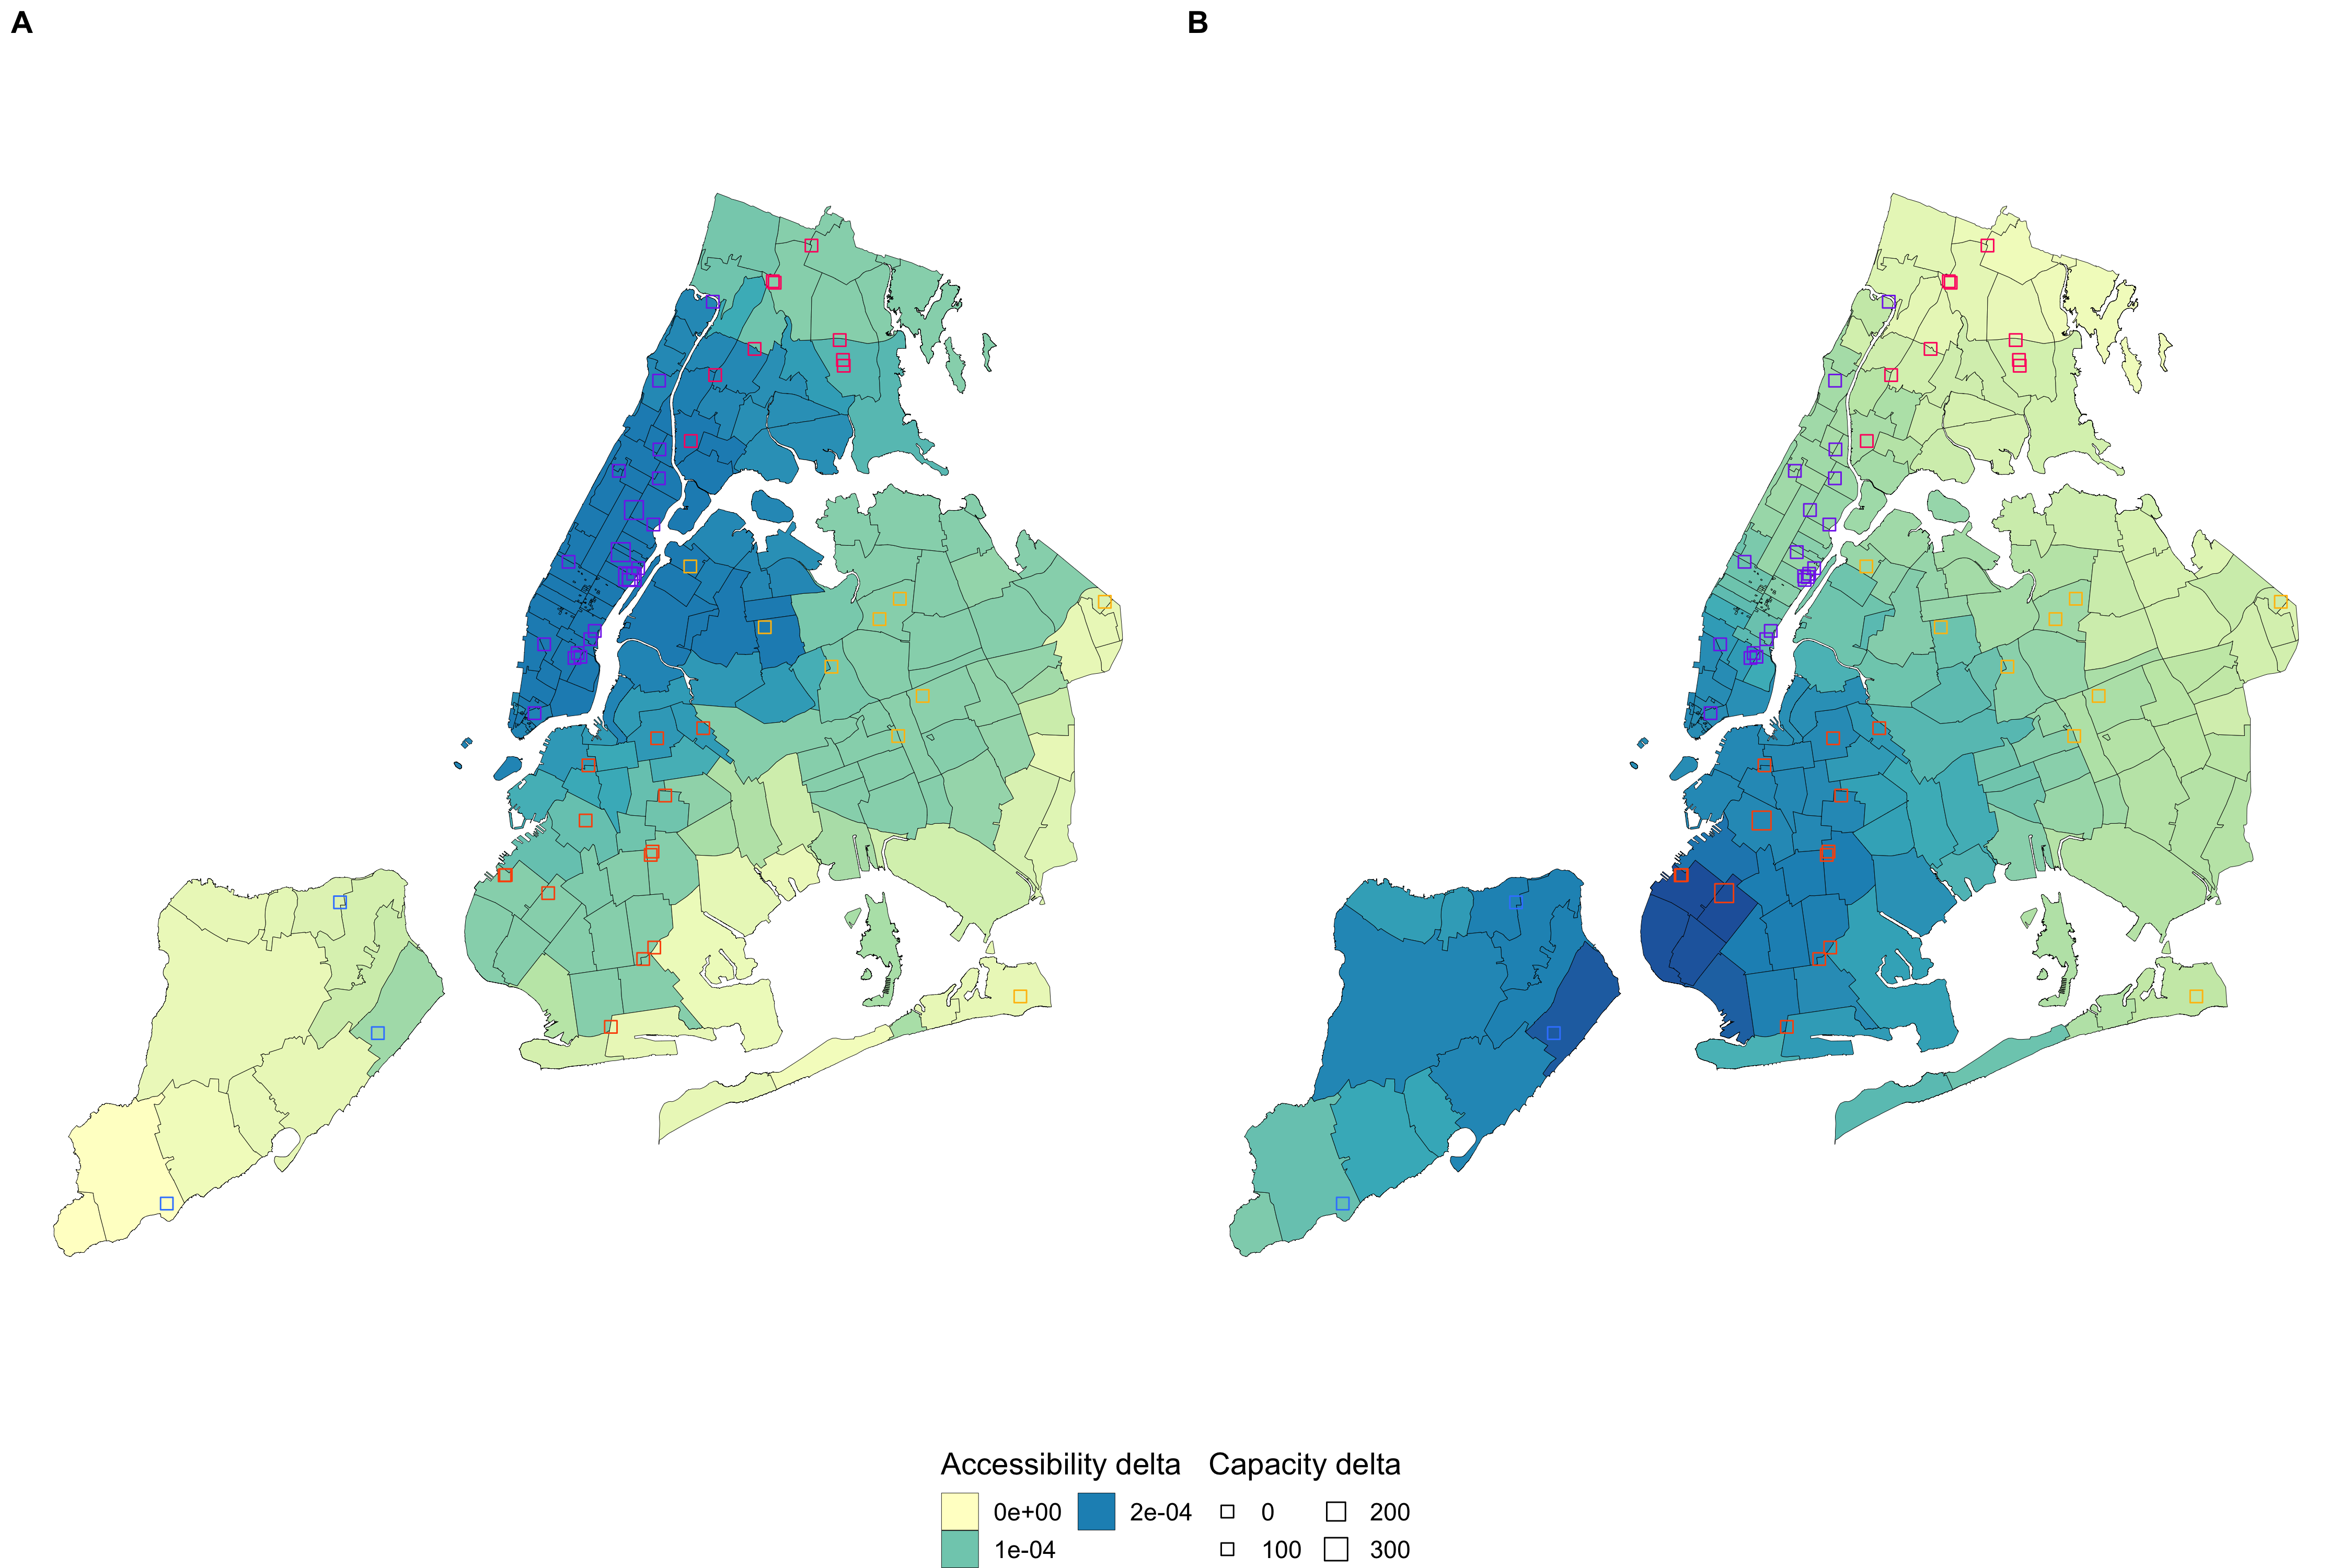
\includegraphics[width=0.9\textwidth]{images/routes/fig3.png}
    \centering
    \caption{ \textbf{\ac{co2} emissions for cancer patients travels} The
        \ac{co2} emissions are computed based on the GPS distance between the
        patient municipality centroid and hospital location. The total emission
        for a single travel is computed as the product of the average \ac{co2}
        emissions per km and the distance. Figure (A) displays the travels
        between municipalities in Ain department. Municipalities are on the
        left, hospitals on the right. Flows are sized by number of travels and
        colored by \ac{co2} emissions. Figure (B) shows the \ac{co2} emissions
        compared with number of stays in Bourg-en-Bresse city (Ain). The
        \ac{co2} emissions are higher for the fewer patients who traveled
        outside of the city to reach more specialized care centers in Lyon. }
    \label{fig:routes-co2-emissions}
\end{figure}

\subsection{Route optimization for cancer patients}

We solved the regularized Optimal Transport problem on the matrix of travel
durations between population locations and hospitals. We used the
\href{https://pythonot.github.io/gen_modules/ot.bregman.html#ot.bregman.sinkhorn}{ot.bregman.sinkhorn}
solver from ``POT: Python Optimal Transport'' \cite{flamary_pot_2021}. The
algorithm performed the patients allocations by minimizing the overall travel
duration while respecting the hospitals maximum capacities. The resulting
allocations are displayed on \cref{fig:sinkhorn-distribution}. Map (A) shows the
allocations in Provence-Alpes-Cote-d'Azur region. Population locations are
displayed as blue triangles, sized by their populations. Hospitals are displayed
as red squares, sized by their capacities. Capacities have been defined as the
number of patients treated by the hospital within the year. The black lines show
the allocations between population locations and patients. The line width is
proportional to the number of patients sent from a population location to an
hospital. Since the algorithm minimized the traveled distance, patients tend to
visit the closer hospitals. Plot
(B) displays the overall traveled distance, and we notice that the optimization
process nearly halved the overall distance. The average traveled distance per
patient went from 34.5 km to 21.9 km, a 36\% decrease. The overall carbon
footprint similarly decreased from 293,009 tons of \ac{co2} to 186,141 tons of
\ac{co2}. We compared the travel distance distribution before the optimization
(C) and after (D), and notice that very few patients travel further than 250 km
with our method.

\begin{figure}[h!]
    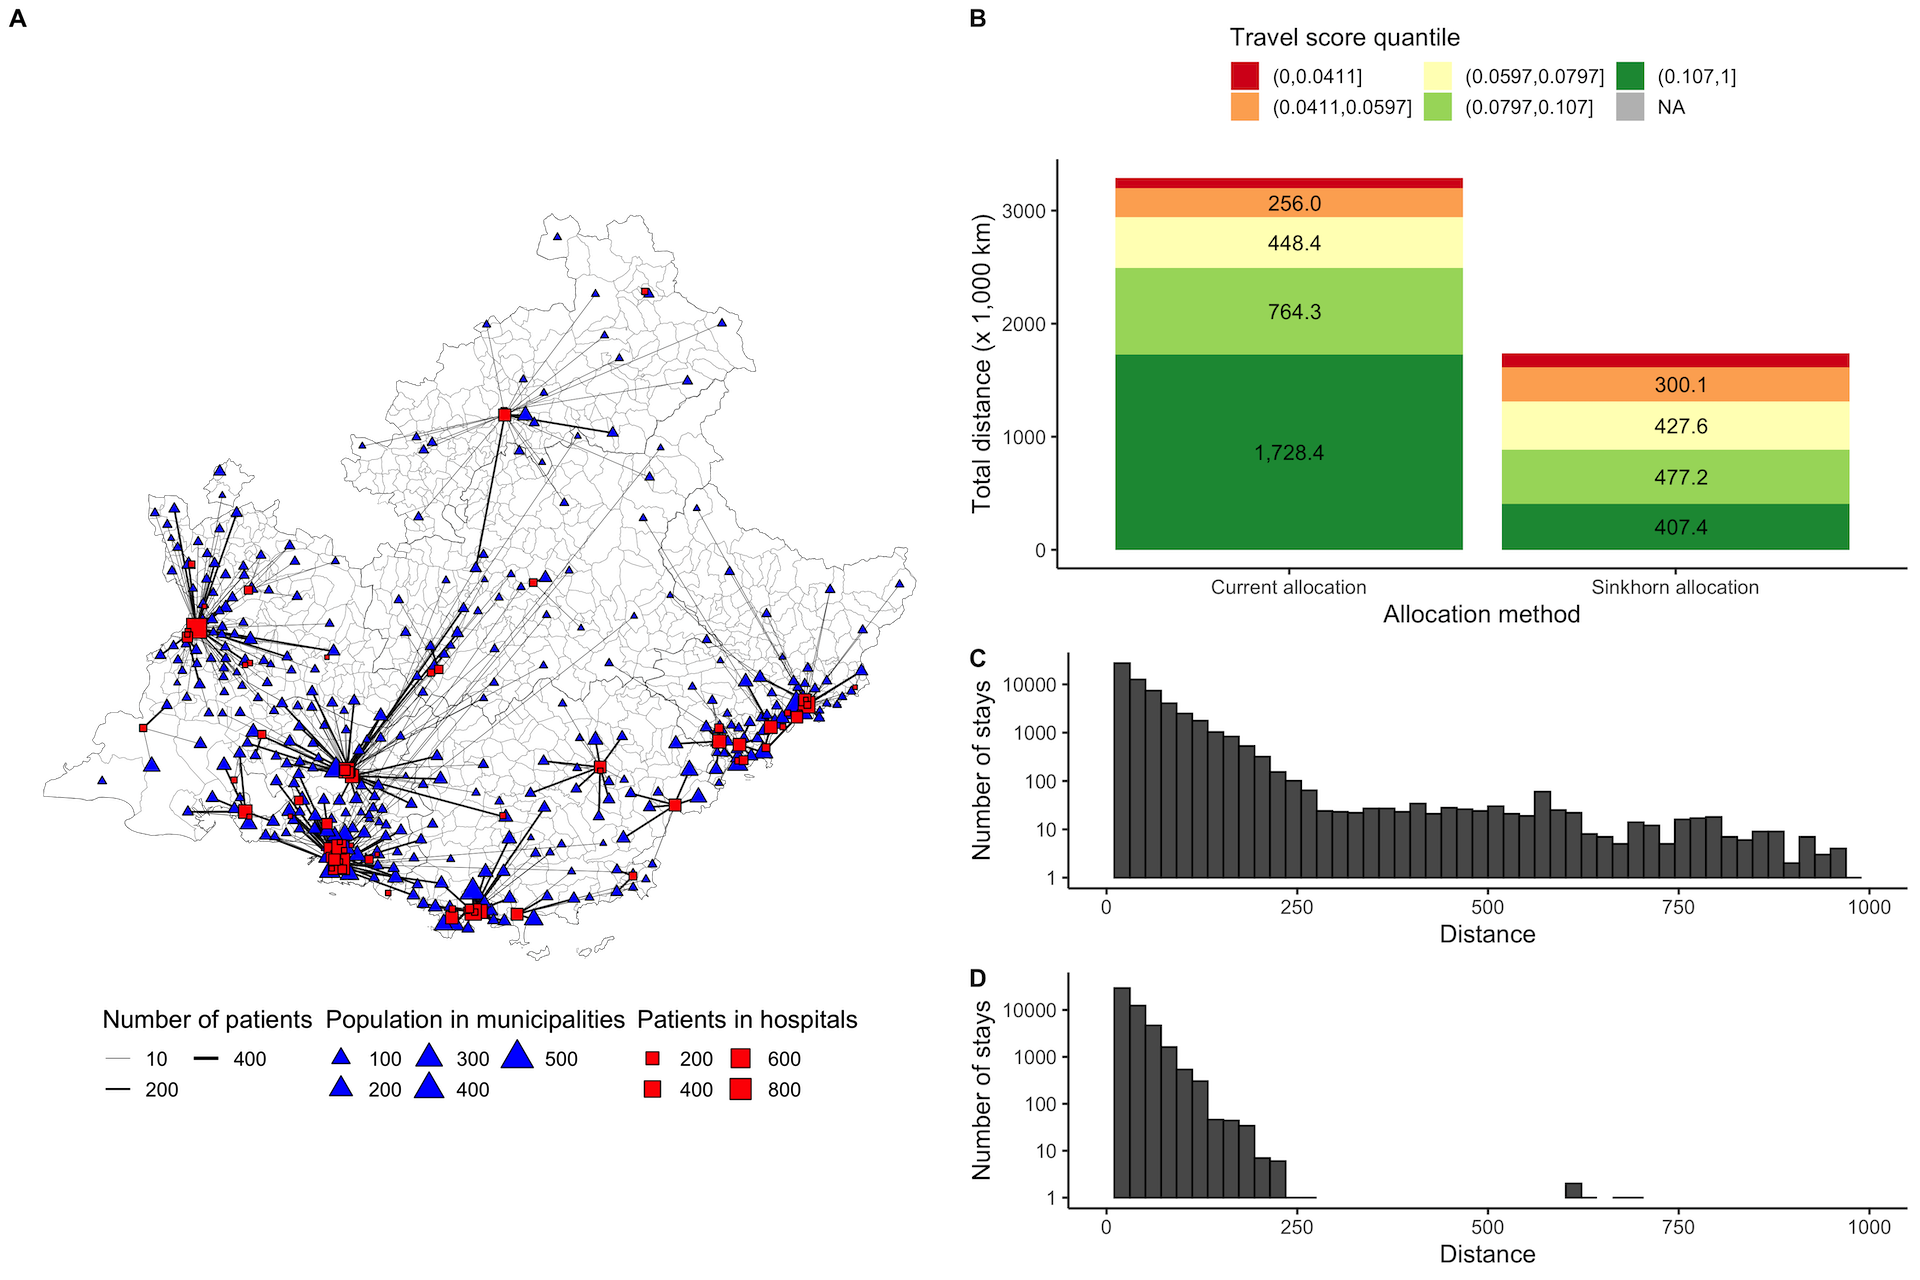
\includegraphics[width=0.9\textwidth]{images/routes/fig10.png}
    \centering
    \caption{ \textbf{Optimization results with the regularized Optimal
            Transport algorithm.} Map (A) shows the allocations in
        Provence-Alpes-Cote-d'Azur region. Population locations are displayed as
        blue triangles, sized by their populations. Hospitals are displayed as red
        squares, sized by their capacities. Plot (B) displays the overall traveled
        distance, and we notice that the optimization process nearly halved the
        overall distance. We compared the travel distance distribution before the optimization
        (C) and after (D), and notice that very few patients travel further than 250
        km with our method.}
    \label{fig:sinkhorn-distribution}
\end{figure}

The alluvial plots on \cref{fig:sinkhorn-alluvium} display the travels flux
between population locations on the right, and hospitals on the left, in the
Bouches du Rhone department (PACA region). The boxes are sized by the number of
patients living in the municipalities and treated in the hospital. The boxes are
sorted by decreasing number of patients. The paths are sized by the number of
patients who traveled from the population location to the hospital, and colored
by the travel burden quantile. The first alluvial plot on the left (A) displays
the routes before the optimization, and the second chart shows the new routing
after the \ac{ot} algorithm (B). Before the optimization process, the travel
burden scores were higher for municipalities with lower populations, i.e.
located to the bottom of the figure. We also notice that the proportion of
patients with more tedious travels is higher for the larger hospitals,
especially ``Institut Paoli-Calmettes'', which is the most specialized in
oncology care within the department. After the optimization algorithm was ran,
the proportion of patients with higher travel burden decreased. We also
notice that patients are routed more homogeneously. Indeed, patients within the
same municipality tend to be sent to the same hospitals.

\begin{figure}[h!]
    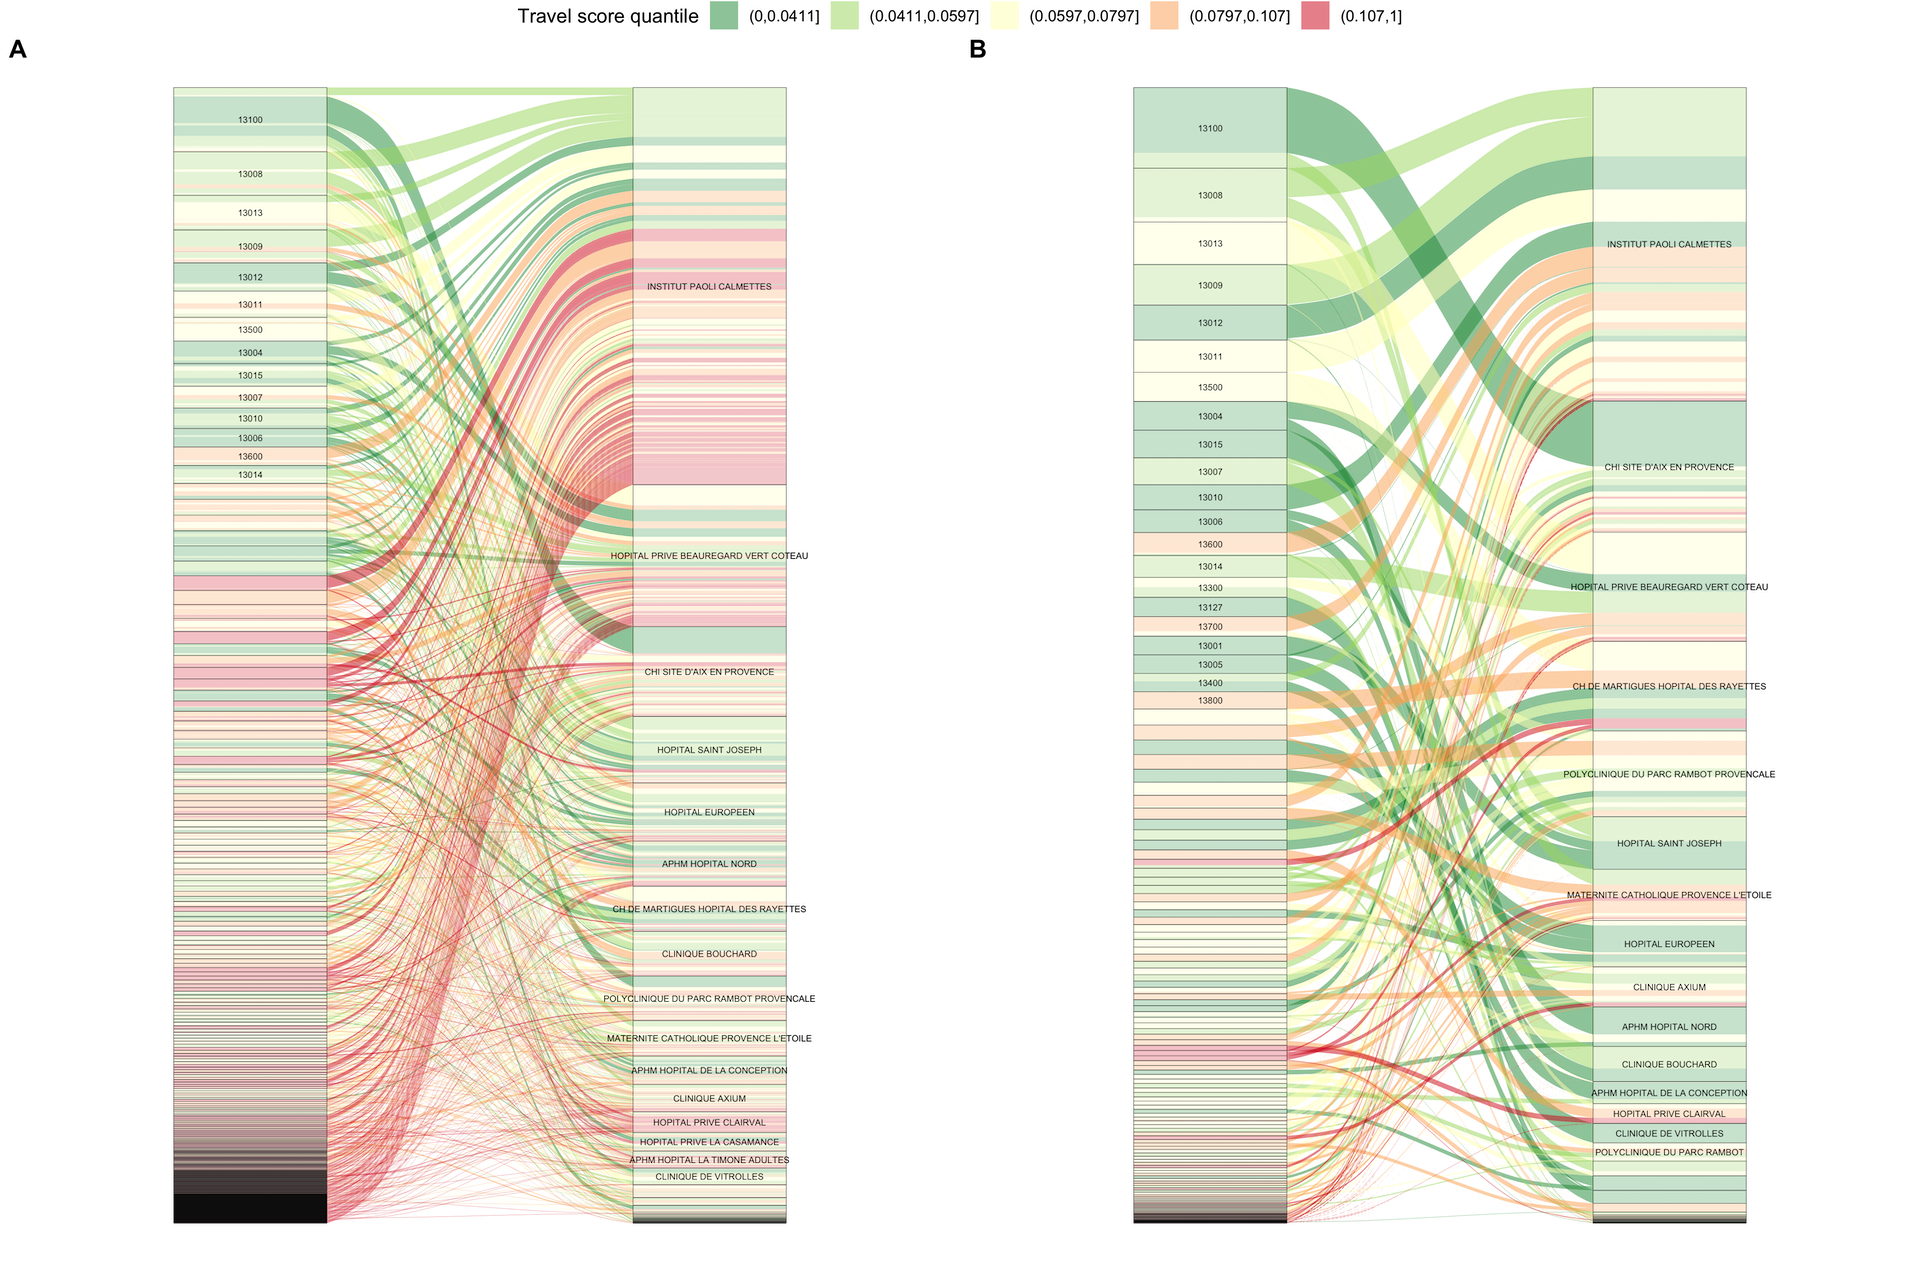
\includegraphics[width=0.9\textwidth]{images/routes/fig11.png}
    \centering
    \caption{ \textbf{Travel flux between in the Bouches du Rhone department
            (PACA region) before and after optimization.} The boxes are sized by
        the number of patients living in the municipalities and treated in
        the hospital. The boxes are sorted by decreasing number of patients.
        The paths are sized by the number of patients who traveled from the
        population location to the hospital, and colored by the travel
        burden quantile. The first alluvial plot on the left (A) displays
        the routes before the optimization, and the second chart shows the
        new routing after the \acf{ot} algorithm (B). }
    \label{fig:sinkhorn-alluvium}
\end{figure}

\section{Conclusion}

We report longer travels for patients living in rural areas. The hospitals
specialized in oncology tend to receive patients from more distant population
locations. Finally, patients with less frequent cancers are forced to travel
further due to the limited number of hospitals that can correctly treat these
pathologies. We introduced the travel burden score, a new metric to consider
when studying patients travels. This score is proportional to not only distance
and duration, but also road sinuosity and number of roundabouts. The last two
variables, which are not explicitly captured by distance and duration, could be
responsible of more tedious drives for the patients, especially when their
health conditions are deprived. In our estimation, the \ac{co2} emissions are
directly proportional to the traveled distance. We did not consider indirect
emissions linked to the transportation. Car was the only transportation mean we
used, and we assumed every patient traveled by car, which might over-estimate
the \ac{co2} emissions. More research is needed to include public transportation
such as train or subway. The larger share of carbon emissions for cancer
surgeries is covered by frequent cancers, that can be treated in many hospitals,
like breast cancer for instance. For such pathologies, a rethink of the
centralization of care model might be needed. Patients from less dense
municipalities could be sent to closer regional hospitals if we make sure the
surgeons' expertise is good enough. Partnerships with larger and more
specialized hospitals could be created to spread the more up to date knowledge
outside the urban hospitals. However, this will be more complicated for rare
cancers, where expertise is scarce and concentrated in the larger hospitals. On
a carbon footprint perspective, we believe the lower number of concerned
patients makes it less of a priority. Finally, we simulated the case where every
patient would travel to the closest hospital, provided we do not exceed the
hospitals maximum capacities. We showed that the average driving distance and
\ac{co2} emissions were reduced by 36\%. While these results are promising, only
minimizing the traveled distance is not sufficient to route the patients to the
optimal hospital. More factors should be taken into account, such as hospital
specialization, quality of care, and detailed patients characteristics. By
comparing the number of patients by hospital before and after the optimization
algorithm, we noticed that the largest and most specialized hospitals received
less patients than before. These hospitals are often saturated, and lowering the
number of patients they receive could benefit them as well as the patients
treated there. These new vacancies could also be filled by patients with more
complicated cases or rare cancers that require a specific expertise that not
every hospital have. We are now interested in the global effects of our
optimization algorithm. A tradeoff should be found between travel distance and
patient-hospital affinity. The case we presented where the patients traveled to
the nearest hospital is the most optimistic situation, and despite this the
driving distance and associated \ac{co2} emissions are ``only'' reduced by 36\%.
Only considered surgery stays were considered here, thus telemedicine will not
be usable to reduce the footprint. The only lever to reduce the associated
carbon footprint is the average \ac{co2} consumption of the driving vehicles,
which will probably drop with the democratization of the electric cars. To sum
up, the results of the travel analysis for cancer patients in metropolitan
France concur with the effects of centralization of care observed in the
literature, where patients living in rural areas tend to experience longer
drives, that are also more tedious.
